\documentclass{beamer}
\usetheme{Madrid}
\usepackage{lmodern}
\usepackage{hyperref}
\usepackage{apacite}
\usepackage[utf8]{inputenc}
\usepackage[spanish]{babel}

\usepackage{xcolor}
\setbeamertemplate{background}{\tikz[overlay,remember picture]\node[opacity=0.2]at (current page.center){
\includegraphics[width=13cm]{KL.png}};}
\usepackage{tikz}
\usepackage{kantlipsum}

\setbeamercolor{normal text}{fg=black}

\begin{document}
\colorlet{beamer@blendedblue}{blue!46!green}
\setbeamercolor{normal text}{fg=black}

\setbeamercolor{frametitle}{fg=white, bg=blue!46!green}
\setbeamercolor*{title}{bg=blue!46!green, fg=white}

\setbeamercolor{section in toc}{fg=black}

\author[Juan C. Correa \textcolor{white}{(\url{https://correajc.com}})]{Juan C. Correa, Ph.D.}
\title[Enseñanza basada en reproducibilidad]{Enseñanza basada en reproducibilidad}
\subtitle{Evaluación Bibliométrica de Literatura Actualizada}
	%\subtitle{}
\institute[]{Fundación Universitaria Konrad Lorenz\\
	\color{blue}\Email  \href{mailto:juanc.correan@konradlorenz.edu.co}{juanc.correan@konradlorenz.edu.co}}
\pgfdeclareimage[height=0.5cm]{KL}{KL}
\logo{\pgfuseimage{KL}}
\setbeamertemplate{caption}[numbered]
\date[Bogotá, Junio-2021]{Curso en: \textbf{T}ecnologías \textbf{R}eproducibles en la \textbf{E}nseñanza de la \textbf{M}etodología y la \textbf{E}stadística}

%\subject{}
\setbeamercolor{background canvas}{bg=white}
%\setbeamertemplate{navigation symbols}{}

\begin{frame}
	\titlepage
\end{frame}

\begin{frame}
\begin{block}{Objetivo del Curso}
\vspace{0.3cm}
Comprender, a través del paquete \textbf{bibliometrix} y la herramienta interactiva \textbf{biblioshiny}, los beneficios de adoptar nuevas tecnologías reproducibles para la enseñanza de contenidos metodológicos y estadísticos orientados al análisis bibliométrico de literatura especializada en cualquier área del conocimiento.
\end{block}
\end{frame}



\begin{frame}
\frametitle{Agenda} 
\tableofcontents
\end{frame}

\section{Justificación de la herramienta}
\begin{frame}{Justificación de la herramienta}
\tiny{\textcolor{blue}{\url{http://dx.doi.org/10.1016/j.joi.2017.08.007}}}
\begin{figure}
\centering

\includegraphics[width=.9\textwidth]{bibliometrix.png}
\end{figure}
\cite{Aria2017}
\end{frame}

\begin{frame}{Justificación de la Herramienta}
``\textit{El número de publicaciones académicas aumenta a un ritmo vertiginoso y cada vez es más inviable permanecer actualizado con todo lo que se está publicando. Además, el énfasis en las contribuciones empíricas ha dado lugar a corrientes de investigación voluminosas y fragmentadas. Esto dificulta la capacidad de acumular conocimientos y recopilar de forma activa las evidencias en trabajos de investigación previos. De allí es que las revisiones de literatura están asumiendo cada vez más un papel crucial en la síntesis de los hallazgos de investigaciones para utilizar de manera efectiva la base de conocimientos existente, avanzar en una línea de investigación y proporcionar una visión basada en la evidencia sobre la práctica de ejercer y mantener el juicio y la experiencia profesional.}''\\
\cite[p. 959]{Aria2017}
\end{frame}

\section{Requerimientos Técnicos}
\begin{frame}{Requerimientos Técnicos}
Para seguir el paso a paso de este tutorial, es necesario que usted haya instalado R y Rstudio en su computador. Acá tiene un video tutorial que le indica cómo hacerlo (\textcolor{blue}{\url{https://youtu.be/Bg2LzHmPZFY}}).
\begin{figure}
\centering

\includegraphics[width=.7\textwidth]{Chupitos.png}
\end{figure}      
\end{frame}

\section{biblioshiny: Tutorial paso-a-paso}
\begin{frame}
\Huge
\centering
\texttt{biblioshiny} \\
Tutorial Paso-a-Paso\\
(En Rstudio Escritorio)
\end{frame}


\begin{frame}{biblioshiny: Paso 1}
Ingresamos a RStudio 
\begin{figure}
\centering
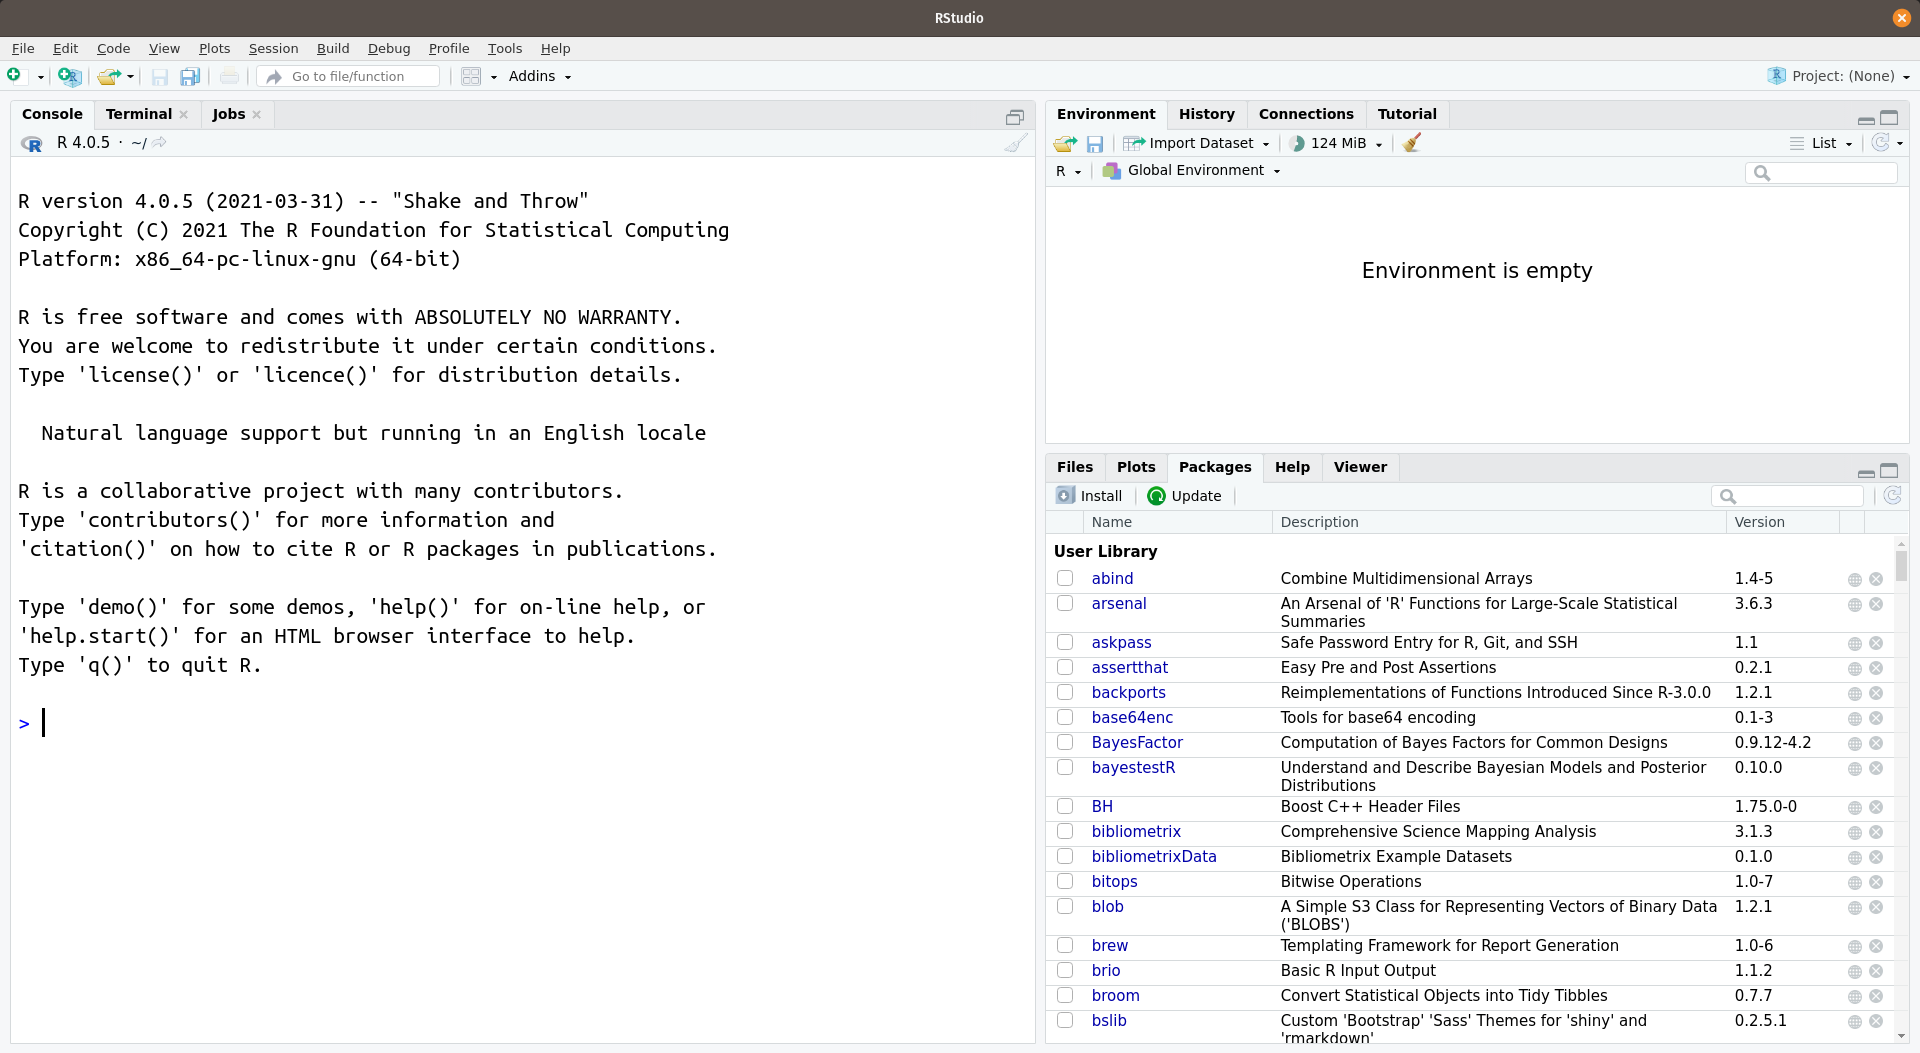
\includegraphics[width=.95\textwidth]{Apariencia.png}
\end{figure}  
\end{frame}

\begin{frame}{biblioshiny: Paso 2}
Vamos a la pestaña Packages
\begin{figure}
\centering
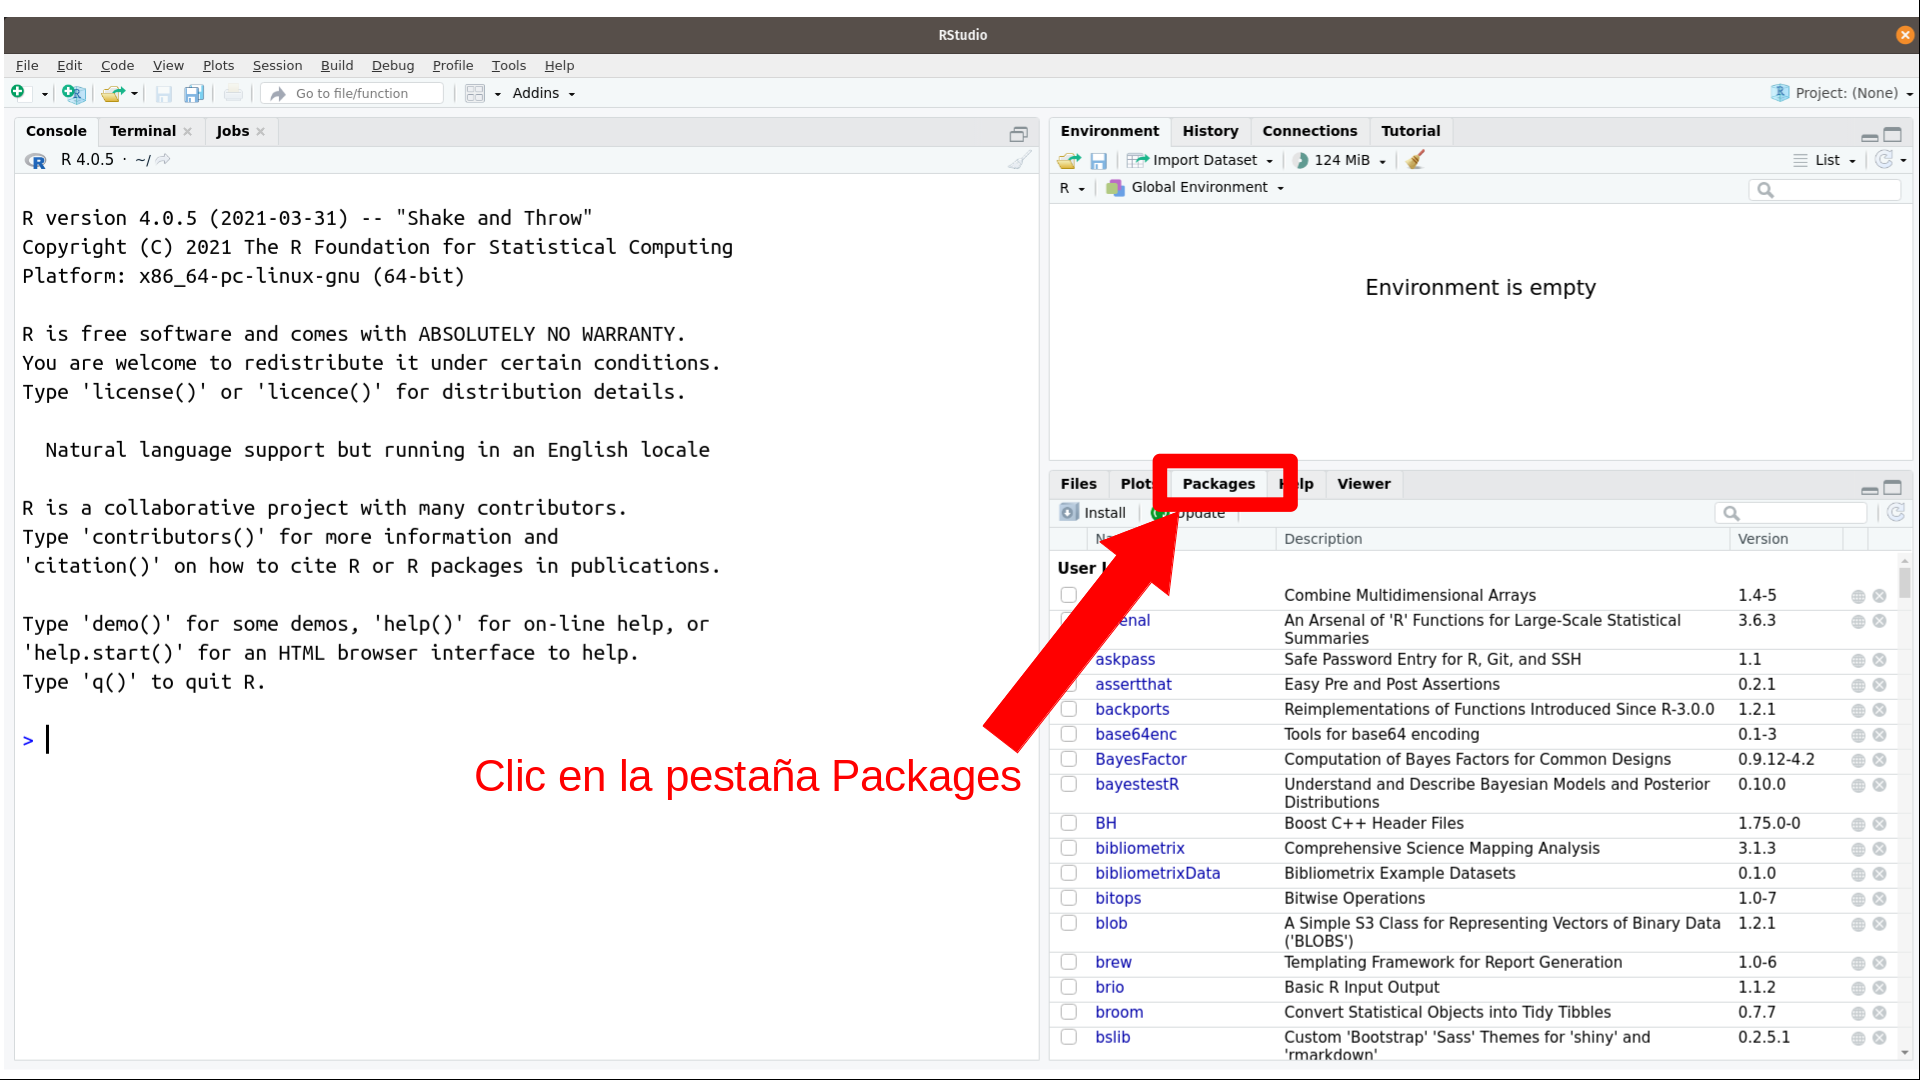
\includegraphics[width=.92\textwidth]{Paso1.png}
\end{figure}  
\end{frame}

\begin{frame}{biblioshiny: Paso 3}
\begin{figure}
\centering
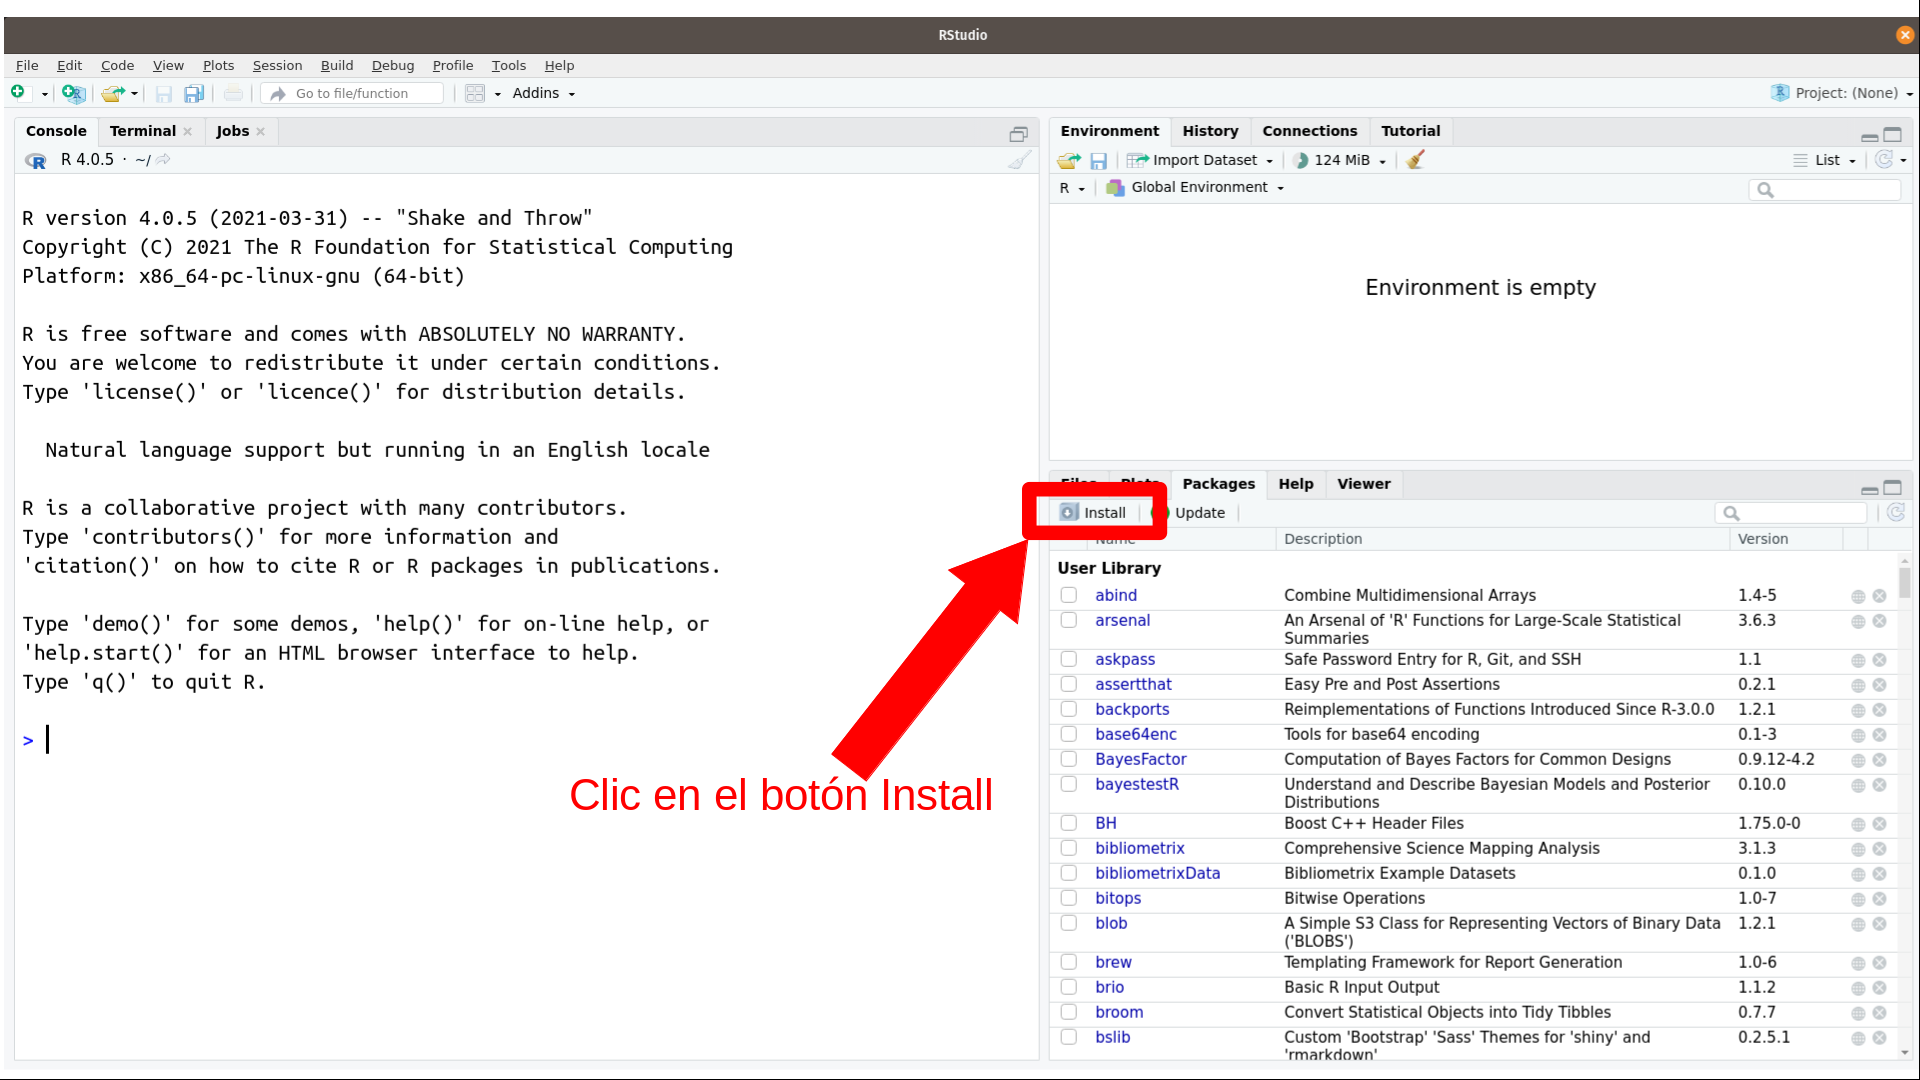
\includegraphics[width=.92\textwidth]{Paso2.png}
\end{figure}  
\end{frame}

\begin{frame}{biblioshiny: Paso 4}
\begin{figure}
\centering
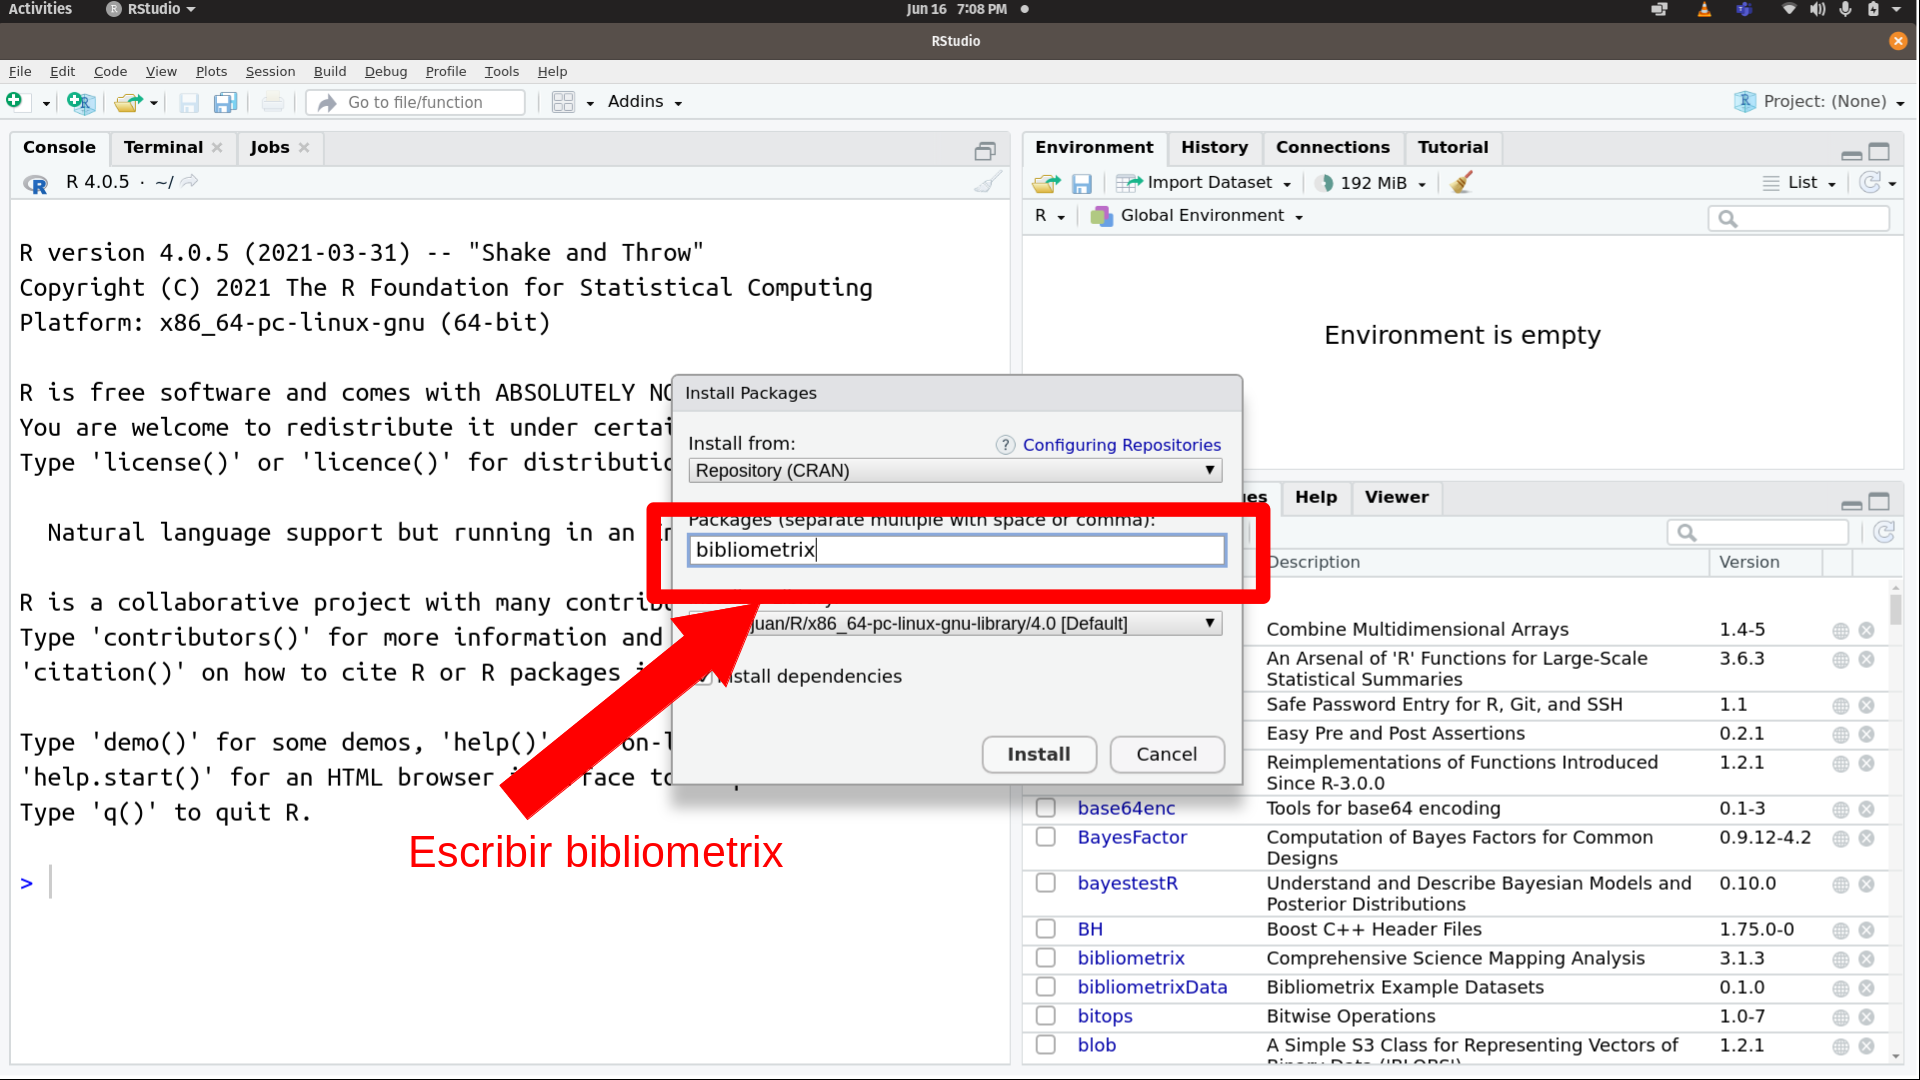
\includegraphics[width=.92\textwidth]{Paso3.png}
\end{figure}  
\end{frame}

\begin{frame}{biblioshiny: Paso 5}
\begin{figure}
\centering
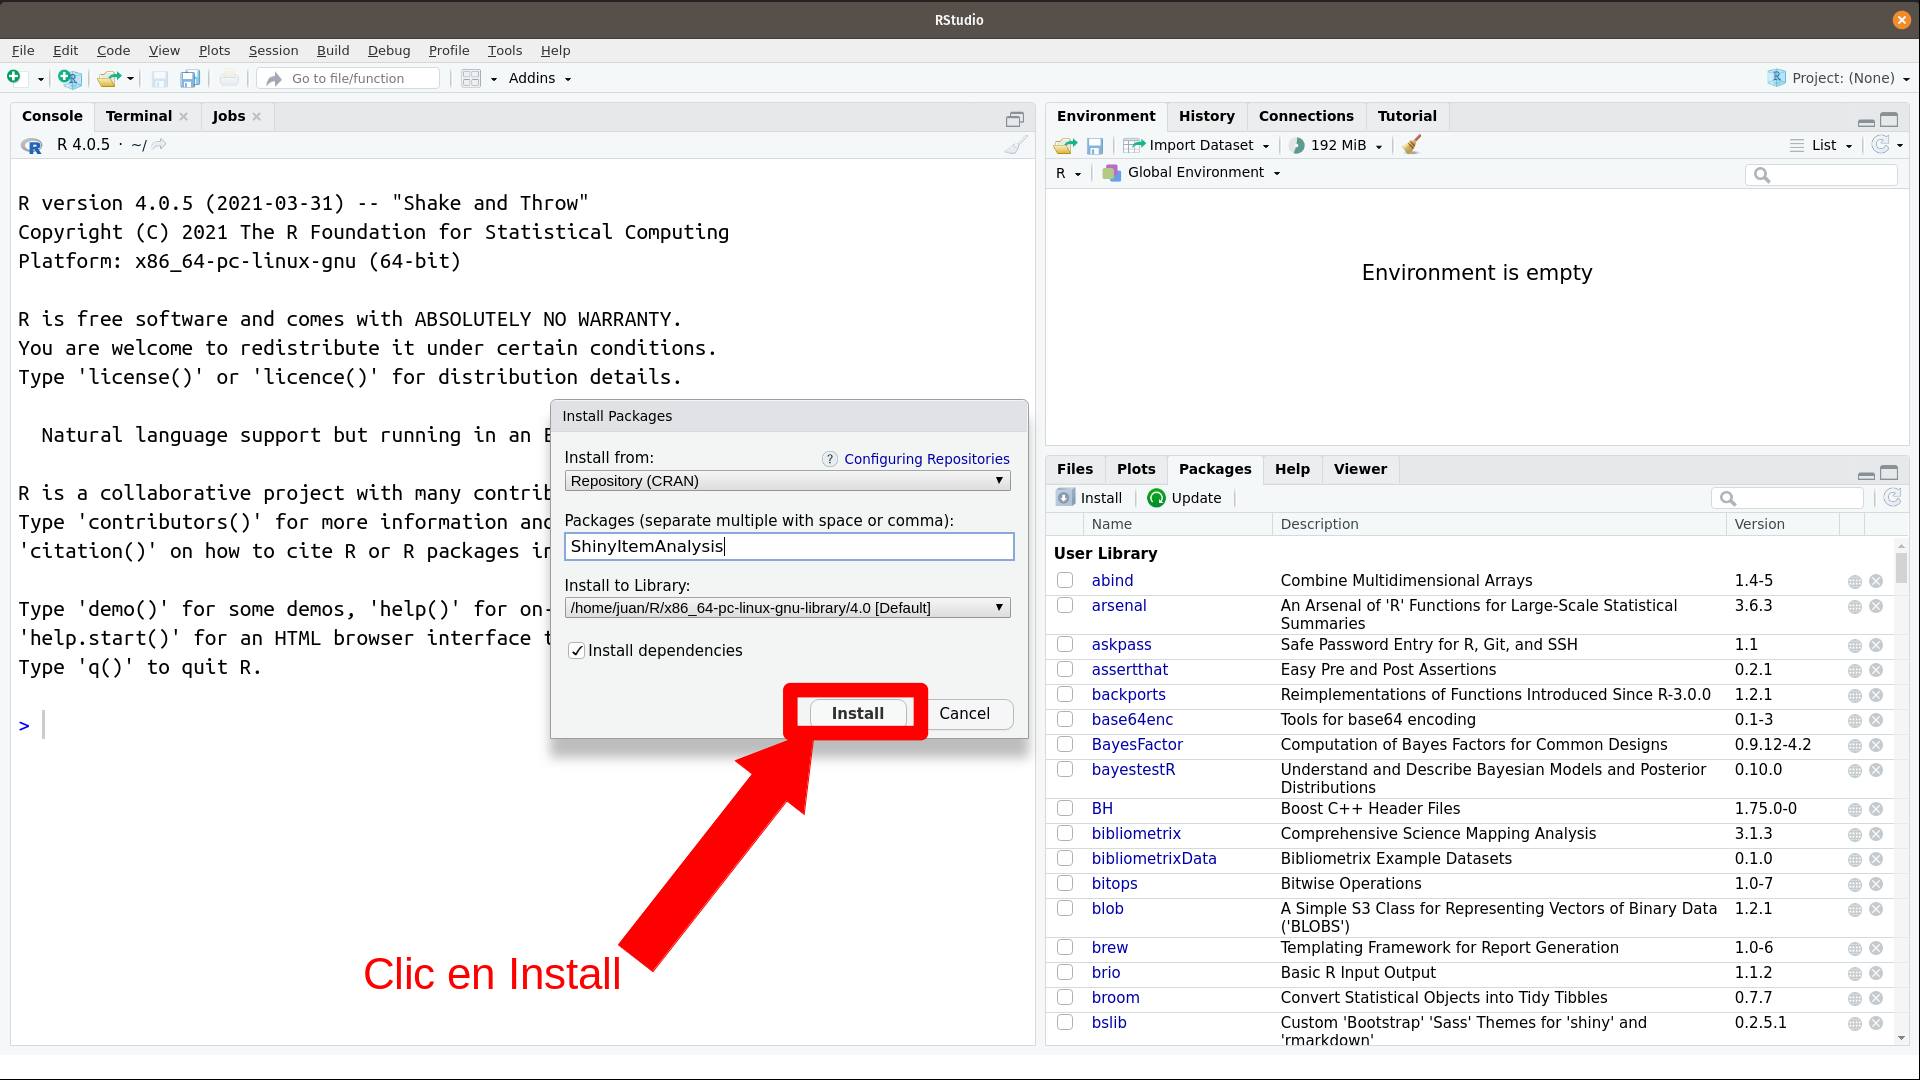
\includegraphics[width=.92\textwidth]{Paso4.png}
\end{figure}  
\end{frame}

\begin{frame}{biblioshiny: Paso 6}
Apariencia de la Console mientras se instala el paquete.
\begin{figure}
\centering
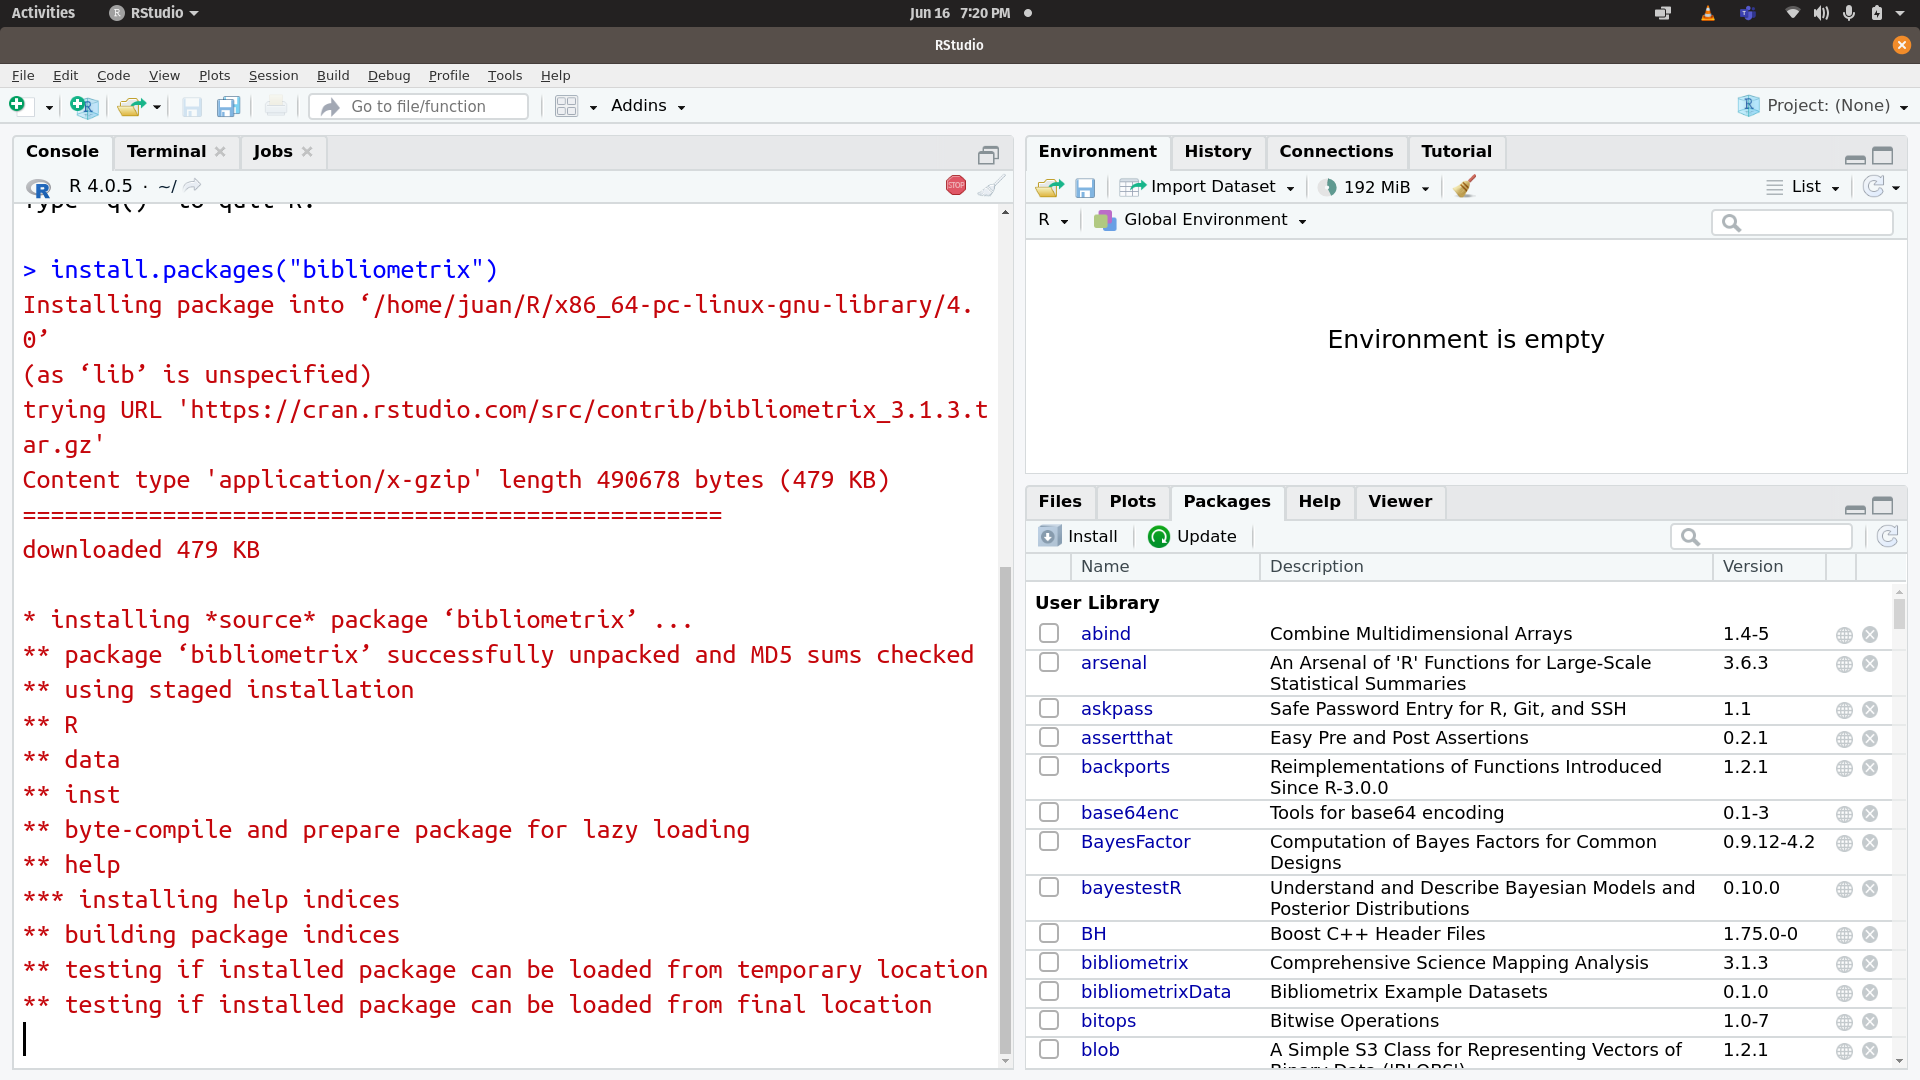
\includegraphics[width=.85\textwidth]{Paso5.png}
\end{figure}  
\end{frame}

\begin{frame}{biblioshiny: Paso 7}
Apariencia de la Console en Rstudio luego de la instalación exitosa del paquete.
\begin{figure}
\centering
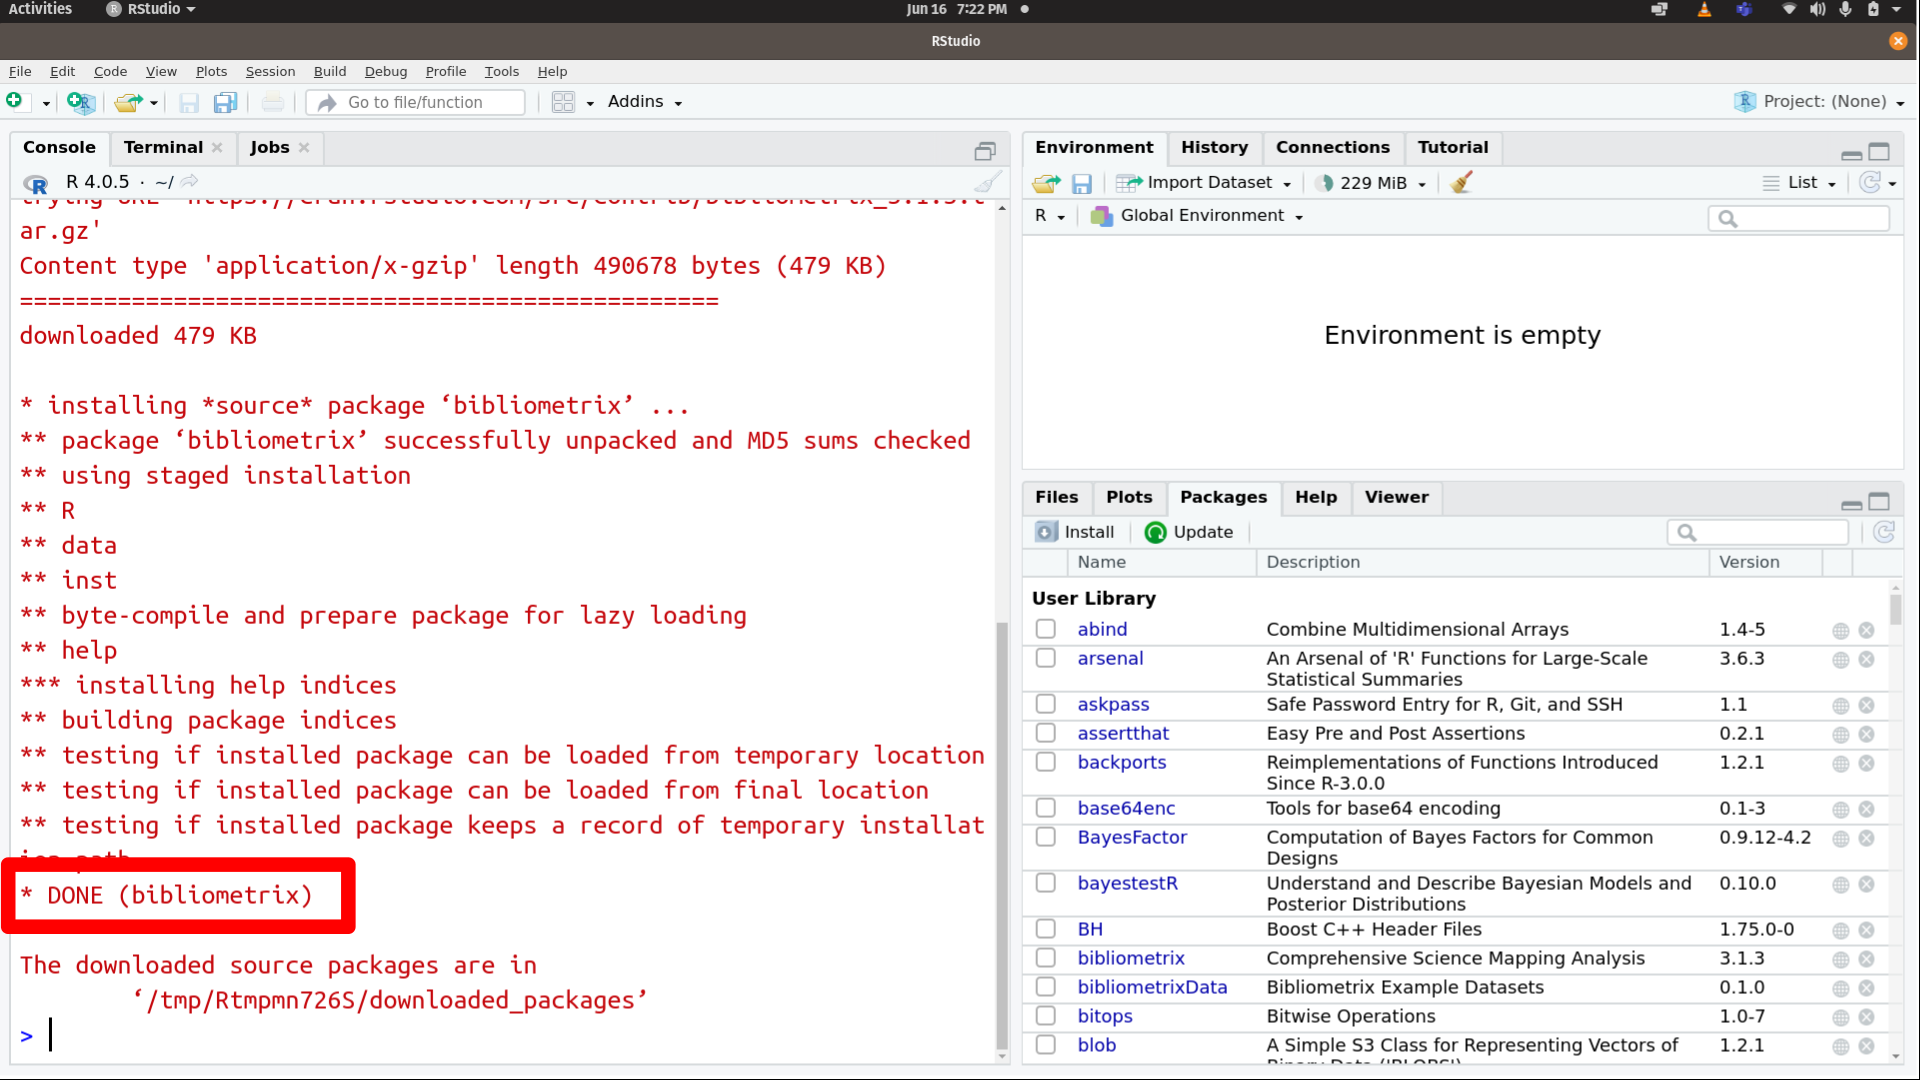
\includegraphics[width=.85\textwidth]{Paso6.png}
\end{figure}  
Verifique la presencia del siguiente mensaje en la Console\\
\textcolor{red}{\texttt{* DONE (bibliometrix)}}
\end{frame}

\begin{frame}{biblioshiny: Paso 8}
Activamos el paquete \texttt{bibliometrix} (haciendo clic en el recuadro al lado izquierdo)
\begin{figure}
\centering
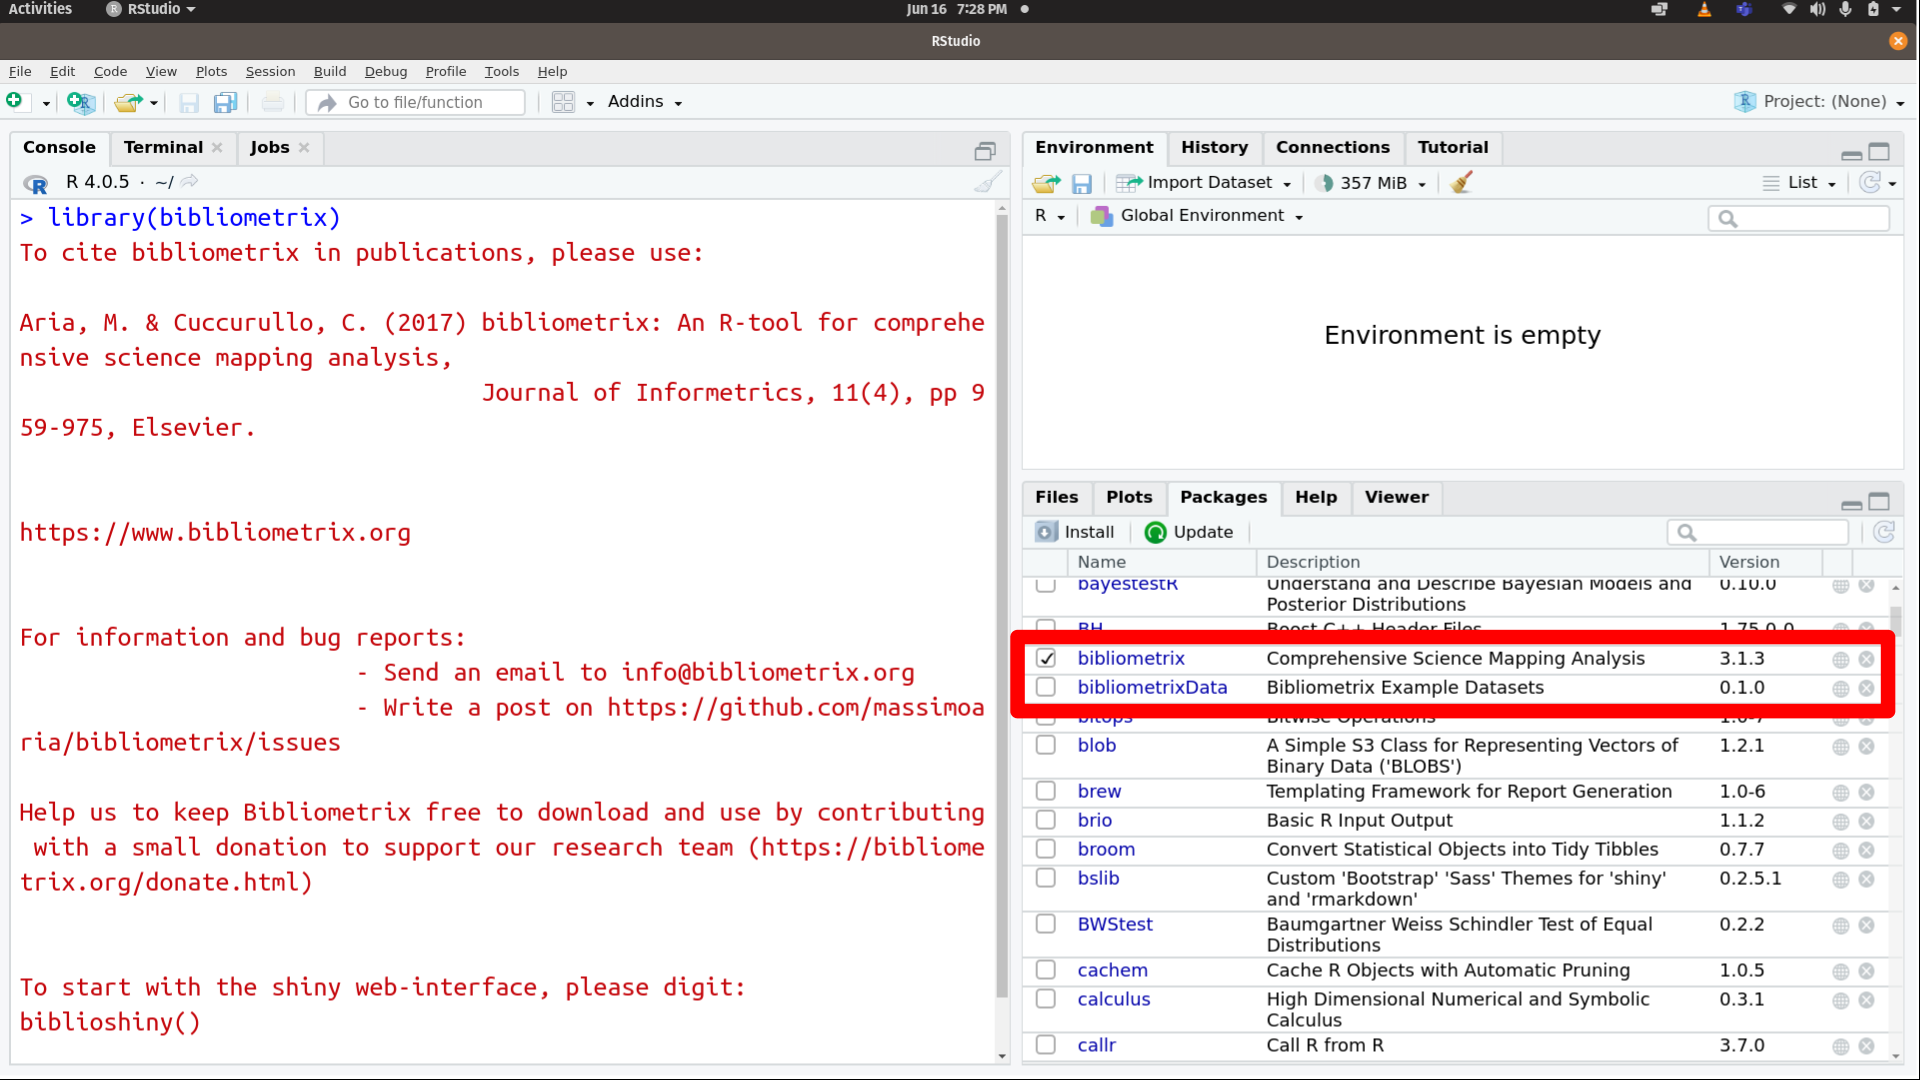
\includegraphics[width=.85\textwidth]{Paso7.png}
\end{figure}  
\end{frame}


\begin{frame}{biblioshiny: Paso 9}
Vamos a ingresar a la herramienta  \texttt{biblioshiny} escribiendo el código \texttt{biblioshiny()}
\begin{figure}
\centering
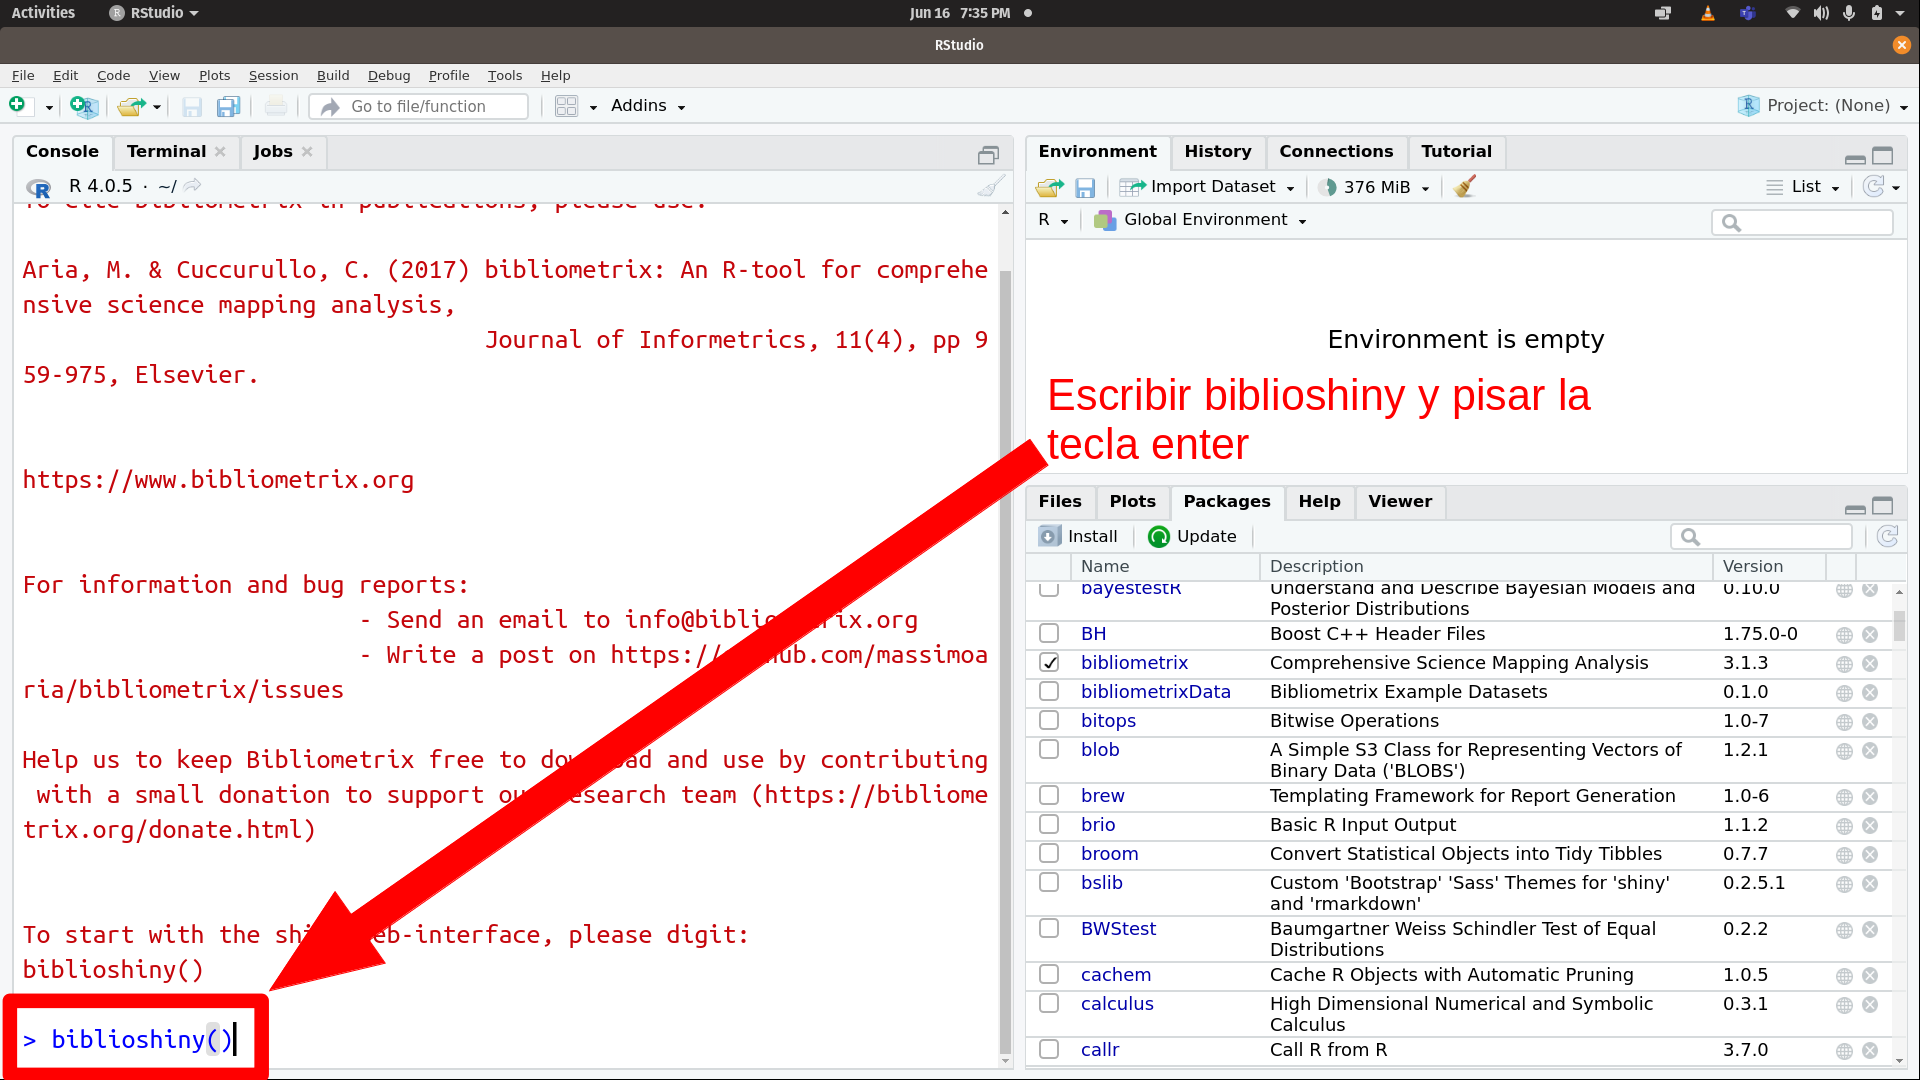
\includegraphics[width=.85\textwidth]{Paso8.png}
\end{figure}  
\end{frame}

\begin{frame}{biblioshiny: Paso 10}
Apariencia de la herramienta \texttt{biblioshiny} dentro de su navegador de Internet
\begin{figure}
\centering
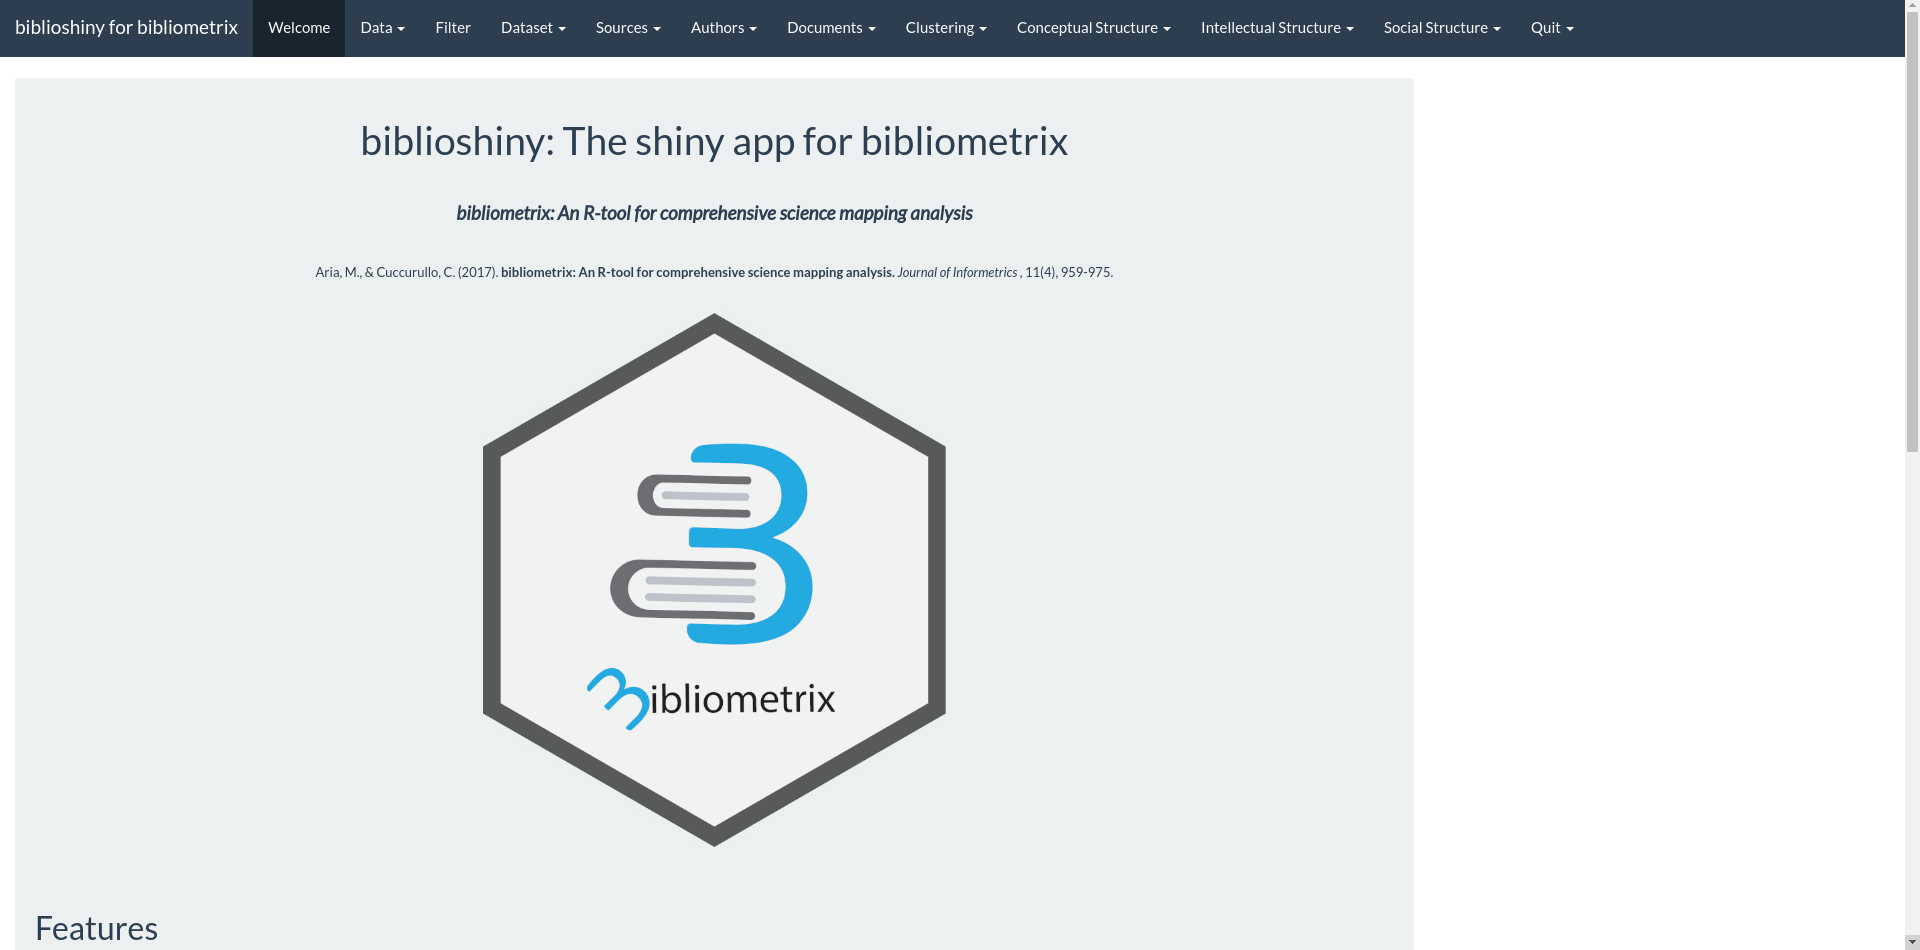
\includegraphics[width=.95\textwidth]{Paso9.png}
\end{figure}  
\end{frame}

\begin{frame}{biblioshiny: Paso 11}
Seleccione los datos que se incluyen de muestra.
\begin{figure}
\centering
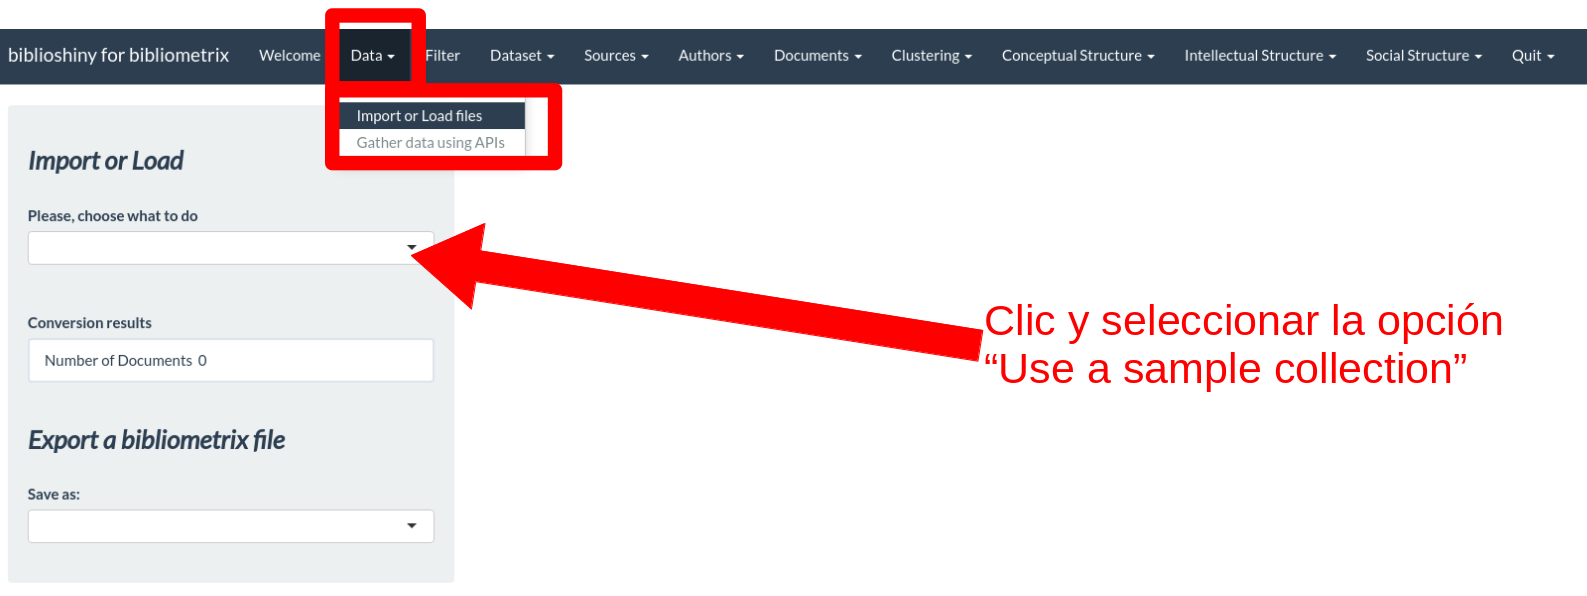
\includegraphics[width=.85\textwidth]{Paso10.png}
\end{figure}  
\end{frame}

\section{biblioshiny adaptado a literatura específica}

\begin{frame}{biblioshiny adaptado a literatura específica}
Antes de usar biblioshiny para analizar literatura actualizada y altamente especializada es necesario saber cómo buscar esta información.
\begin{figure}
\centering
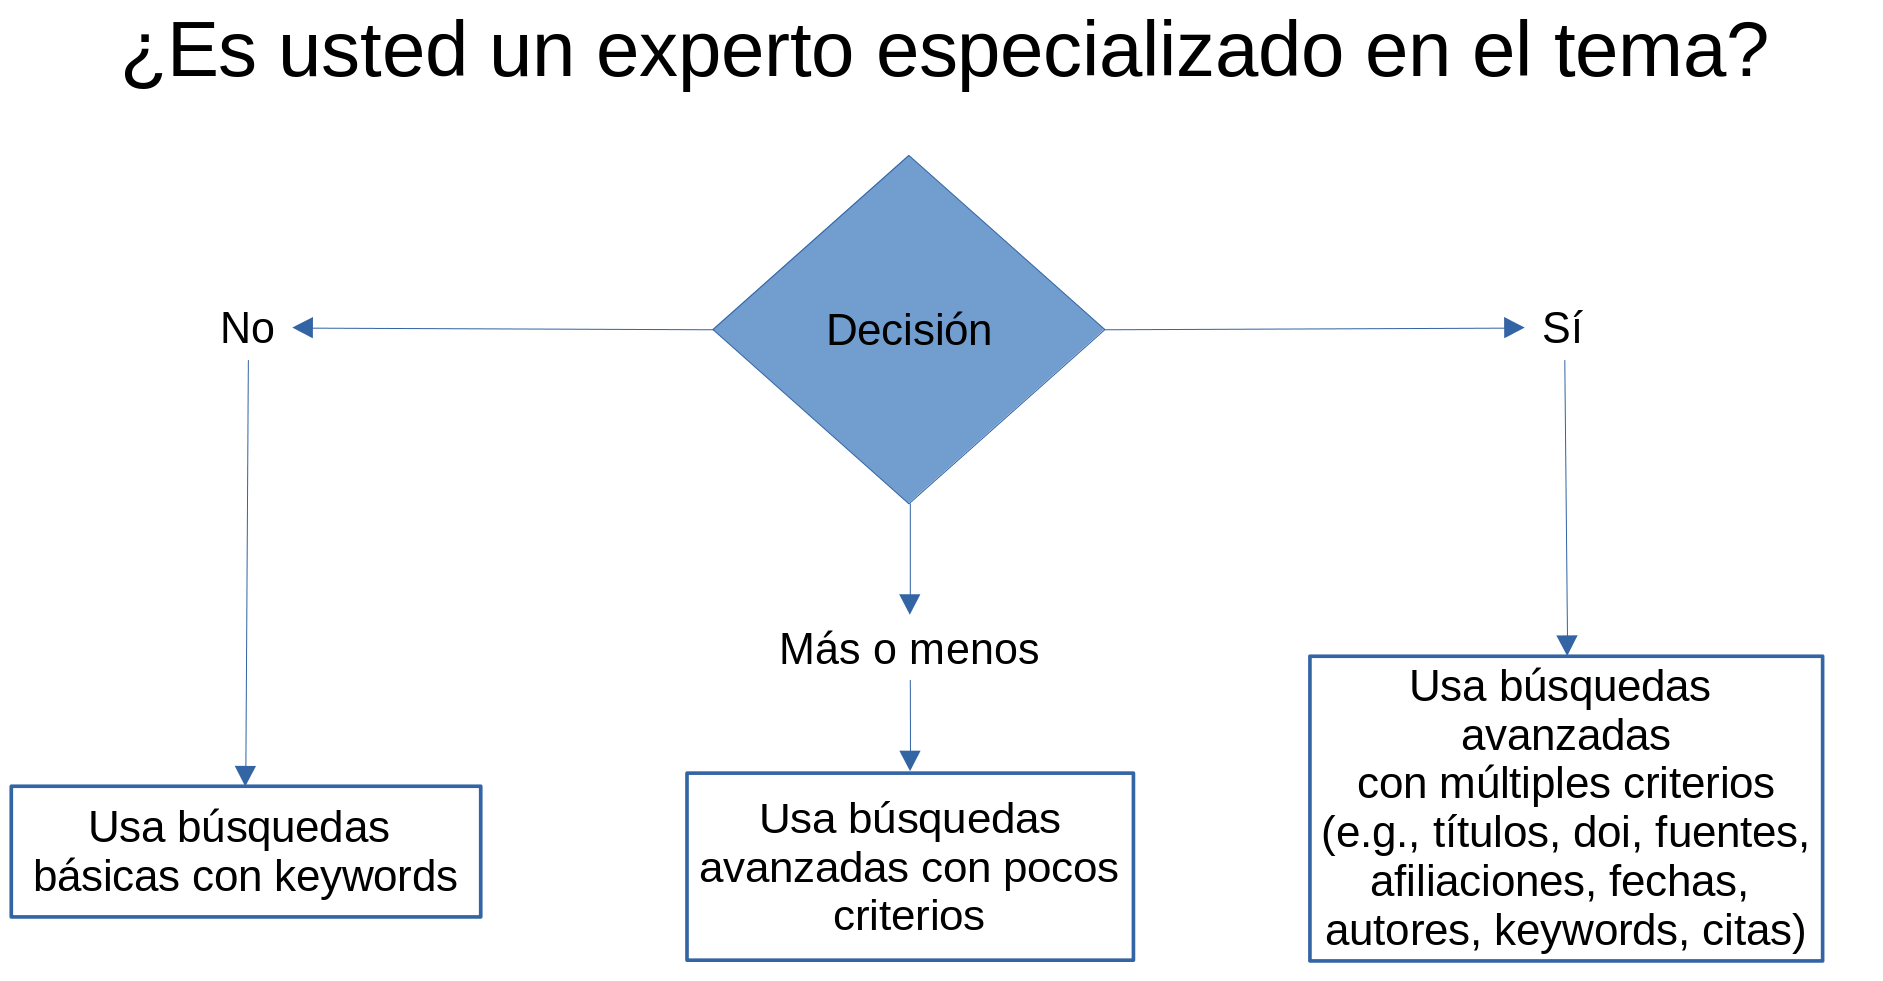
\includegraphics[width=.85\textwidth]{experticia.png}
\end{figure}  
\end{frame}

\begin{frame}{biblioshiny adaptado a literatura específica}
El caso 1 muestra 169 documentos que cumplen con el criterio de búsqueda. El caso 2 muestra 2 documentos que cumplen con los dos criterios de búsqueda. ¿Cuál usar?
\begin{figure}
\centering
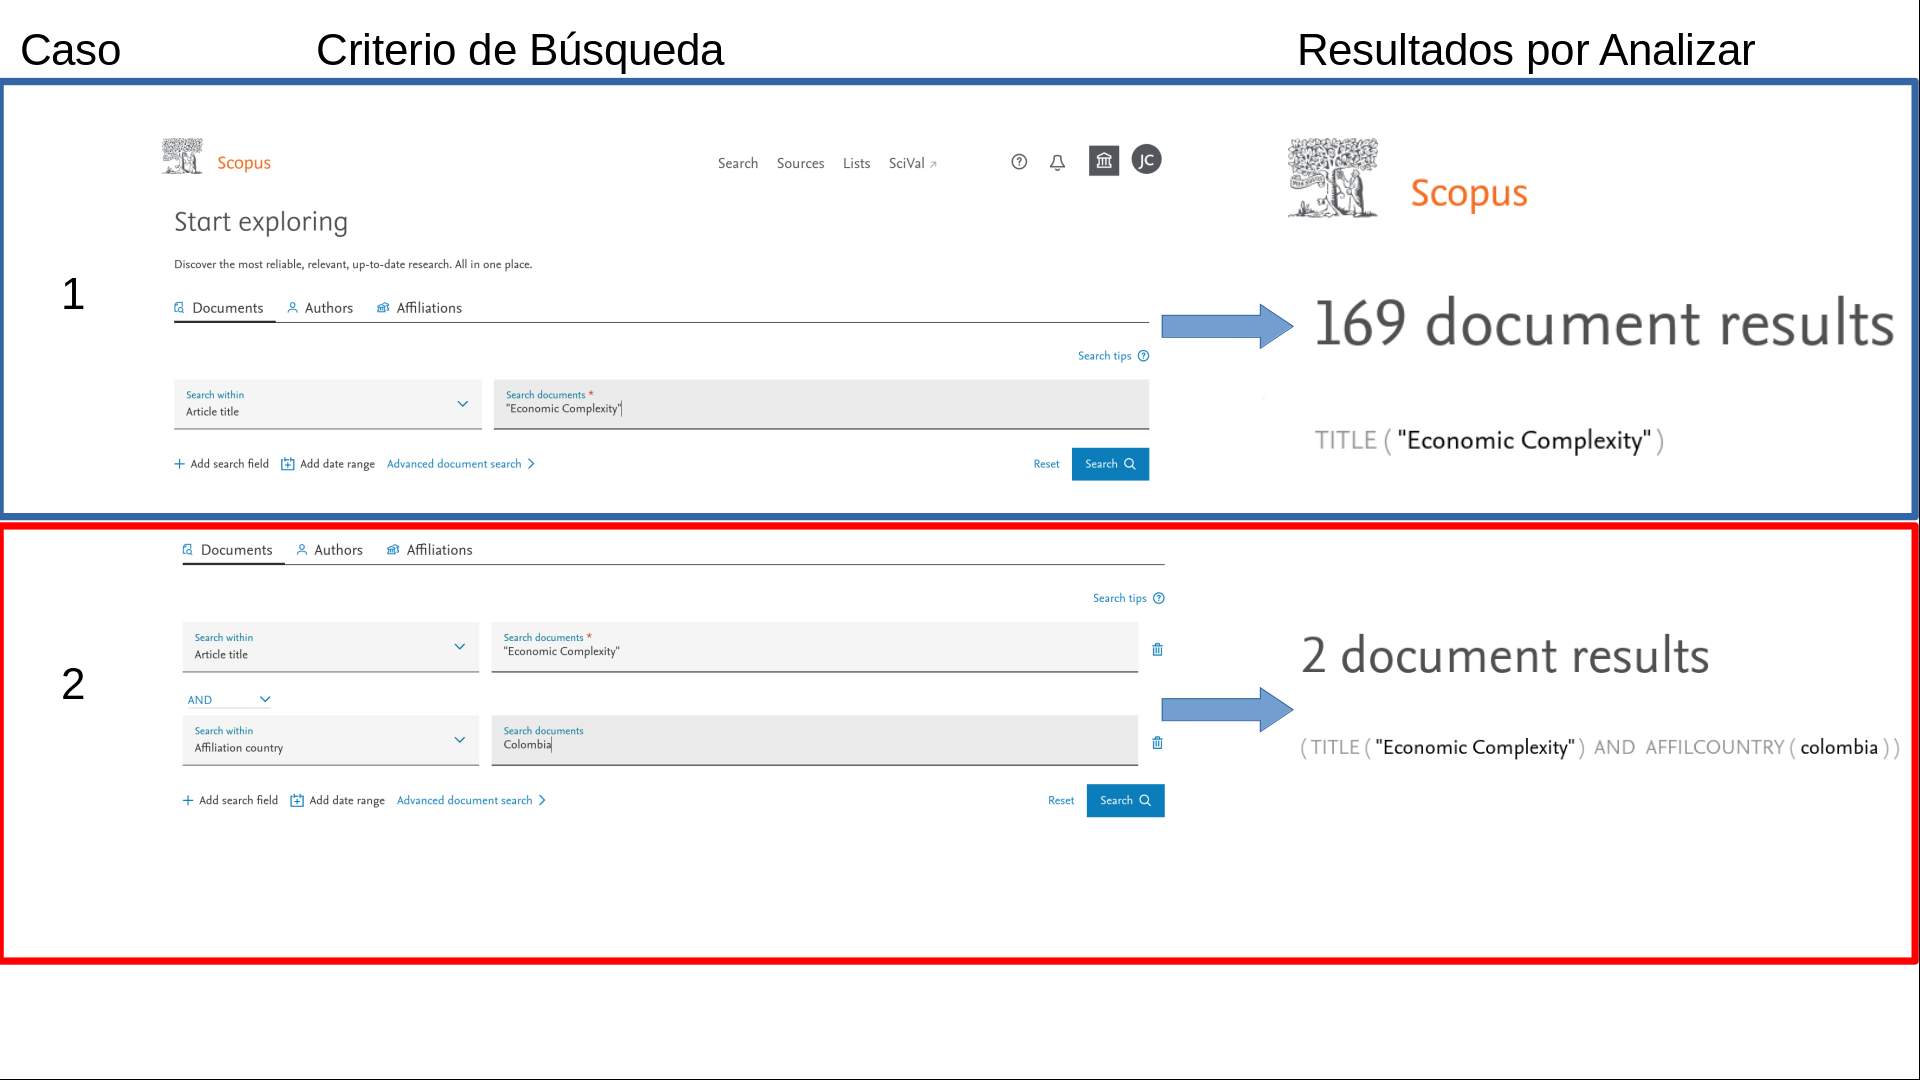
\includegraphics[width=.85\textwidth]{Casos12.png}
\end{figure}  
\end{frame}

\subsection{Ejemplo blockchain}
\begin{frame}{Ejemplo blockchain}
El caso 1 muestra 13.089 documentos que cumplen con el criterio de búsqueda. El caso 2 muestra que al añadir el ISSN de una revista específica, el resultado cambia en tres órdenes de magnitud (i.e., solo 13 documentos). ¿Cuál usar?
\begin{figure}
\centering
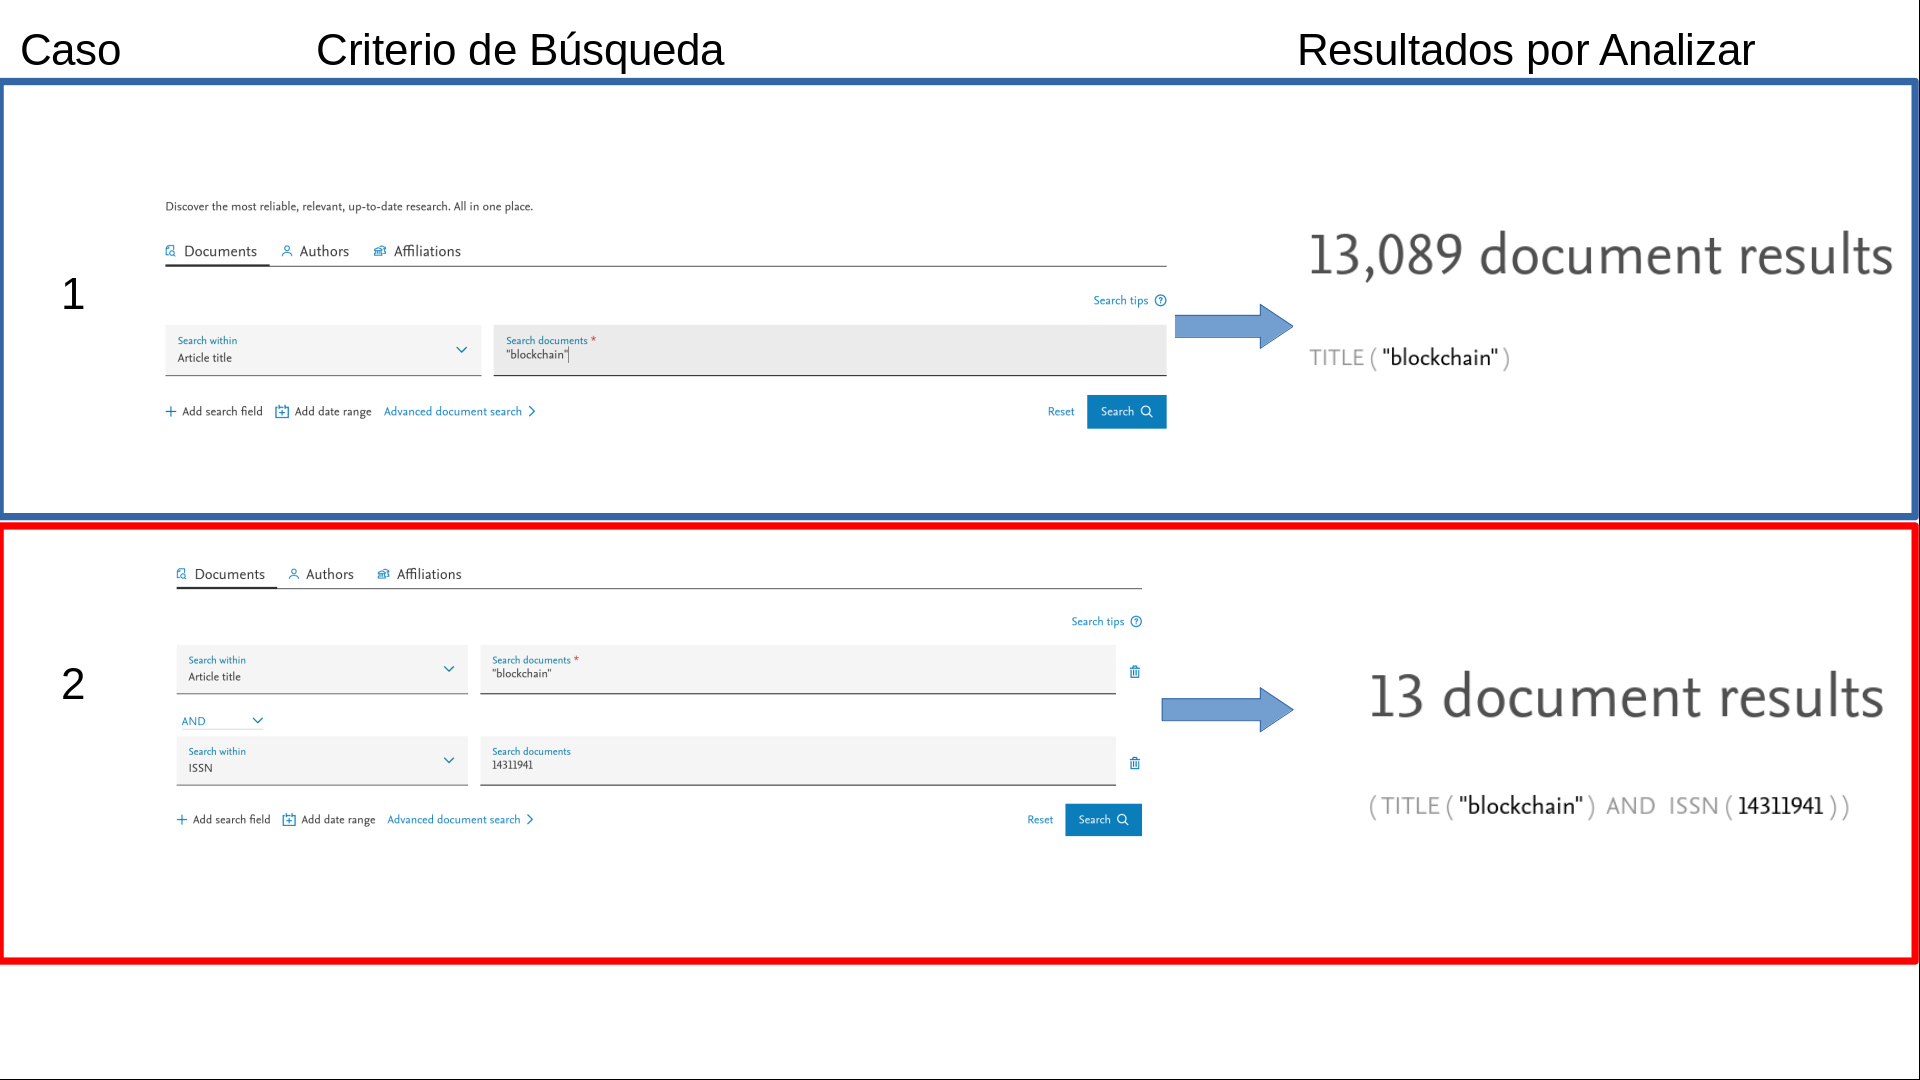
\includegraphics[width=.85\textwidth]{Caso34.png}
\end{figure}  
\end{frame}

\begin{frame}{Ejemplo blockchain}
Veamos qué podemos hacer en biblioshiny para analizar lo publicado sobre blockchain únicamente en el año 2021 por parte de investigadores afiliados a instituciones de China.
\begin{figure}
\centering
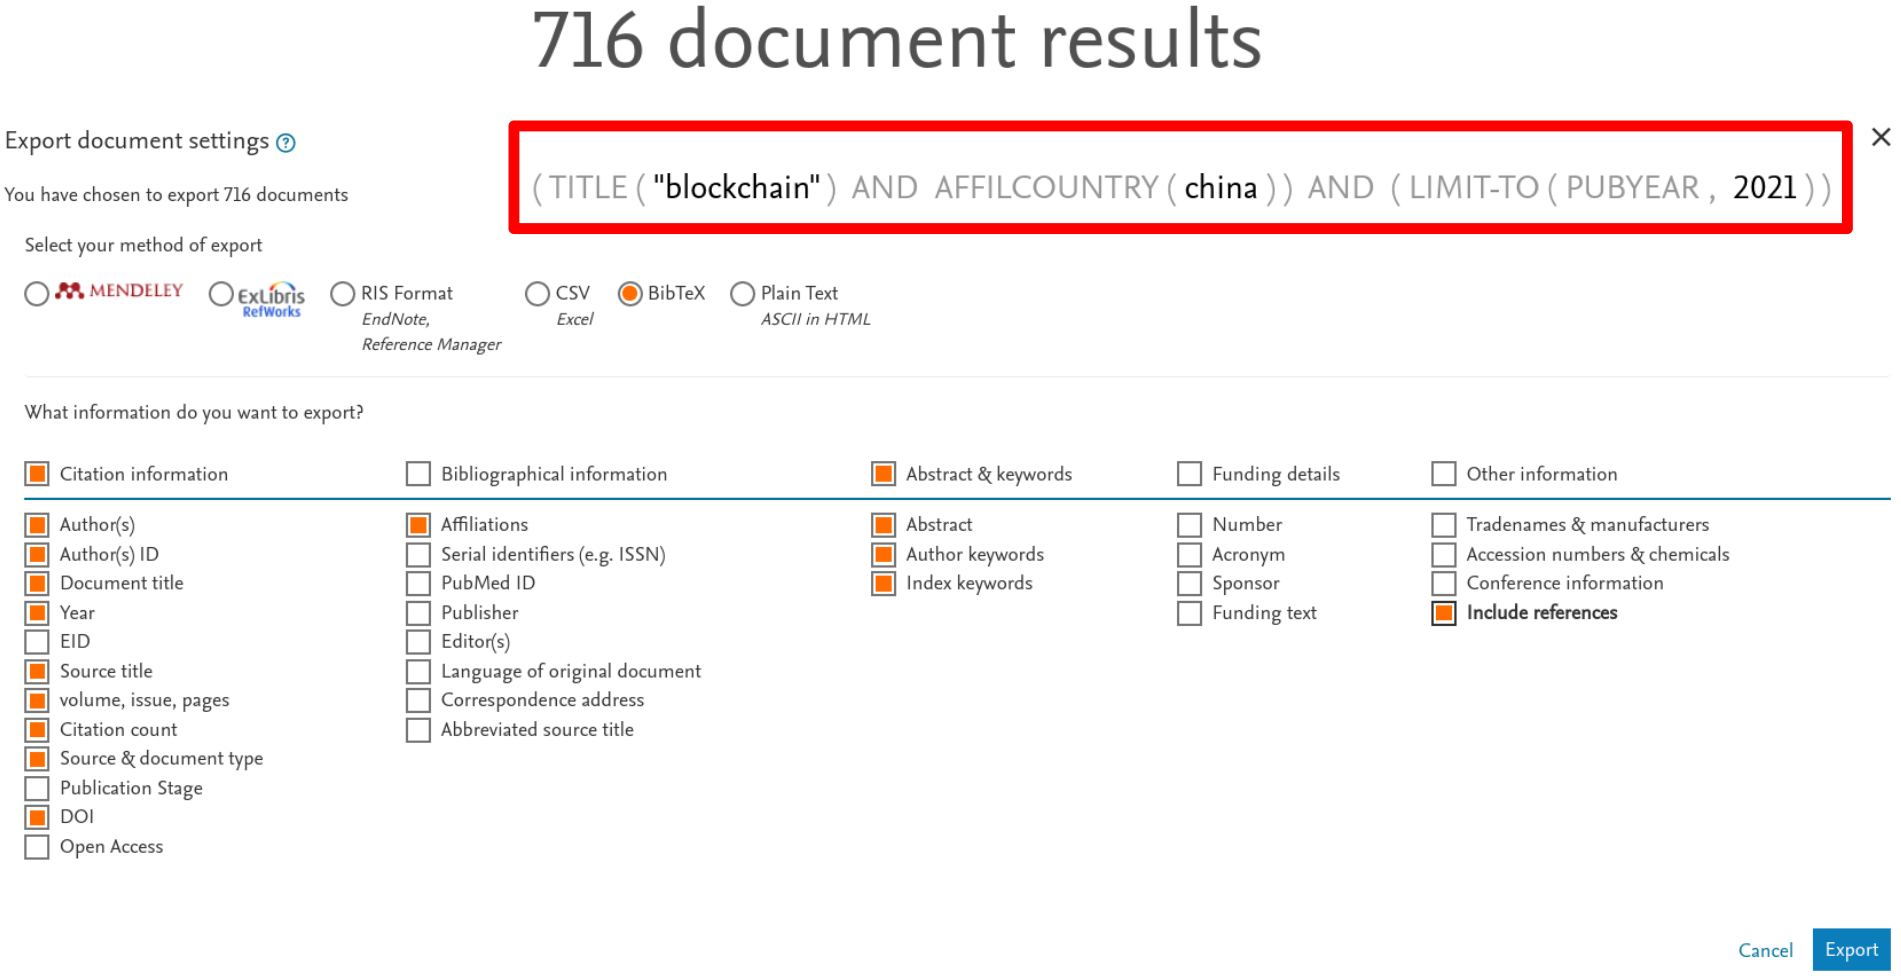
\includegraphics[width=.75\textwidth]{blockchainChina2021.png}
\end{figure}  
Selecciones Bibtex como método de exportación con los campos seleccionados en naranja y presione el botón Export.
\end{frame}

\begin{frame}{Ejemplo blockchain}
Apariencia de \texttt{biblioshiny} luego de haber abierto los datos exitosamente, previamente descargados desde Scopus.
\begin{figure}
\centering
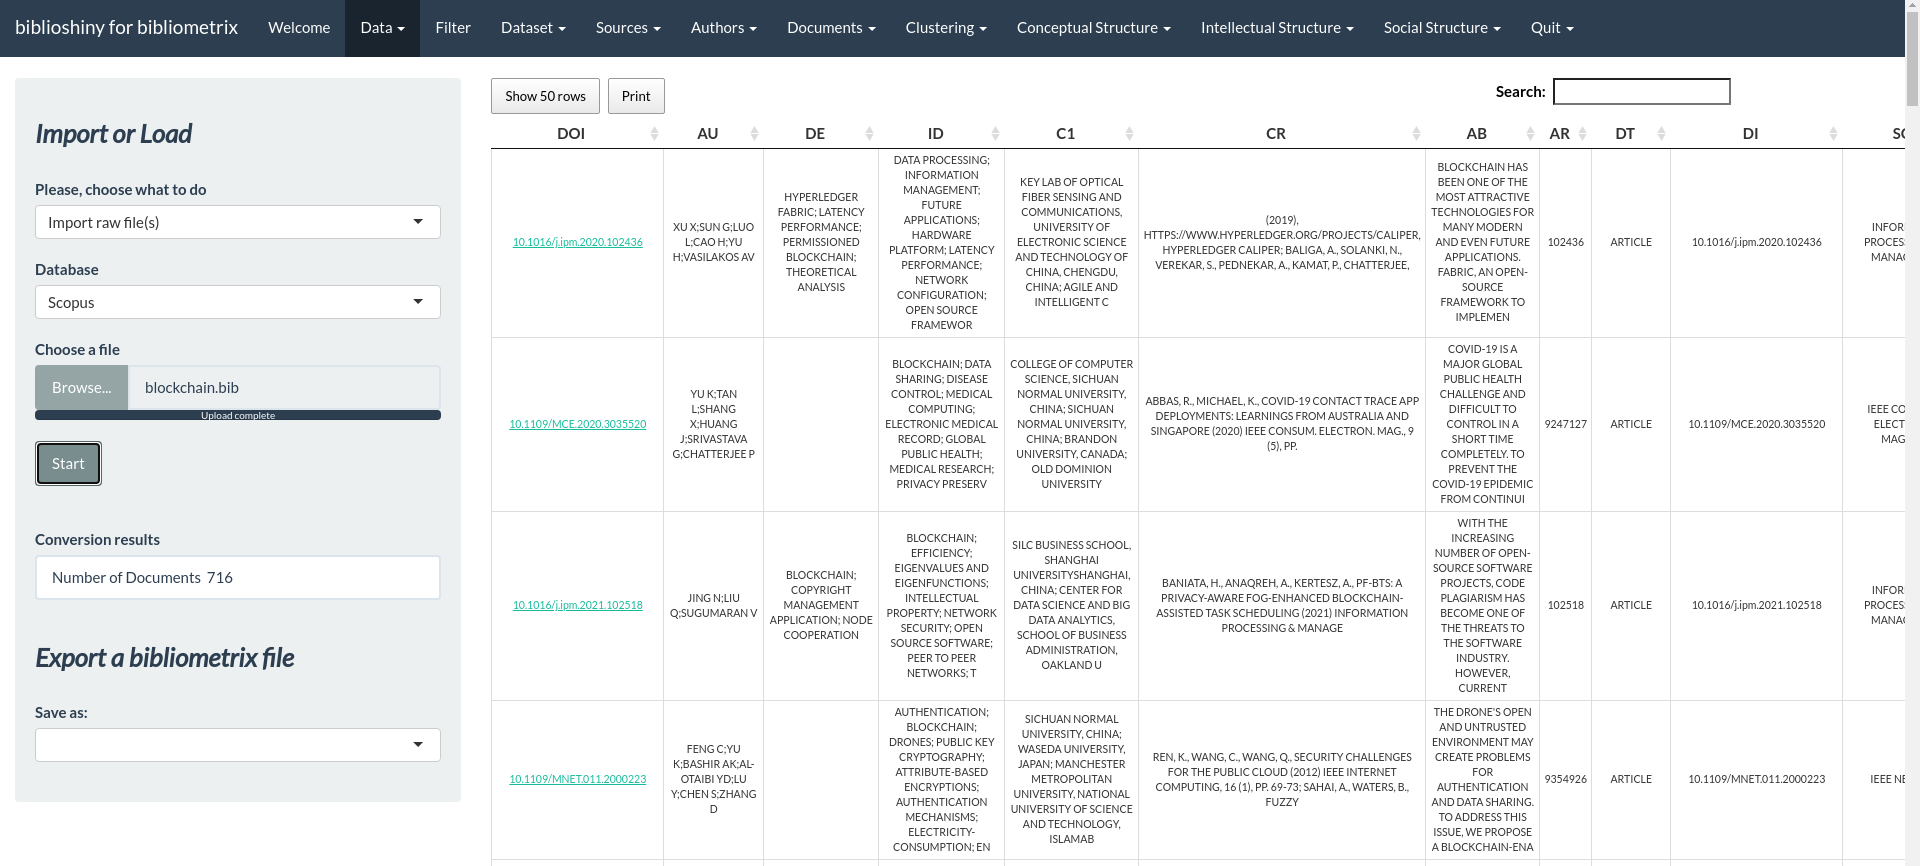
\includegraphics[width=.95\textwidth]{ejemplo1.png}
\end{figure}  
\end{frame}

\begin{frame}{Ejemplo blockchain}
Algunos resultados
\begin{figure}
\centering
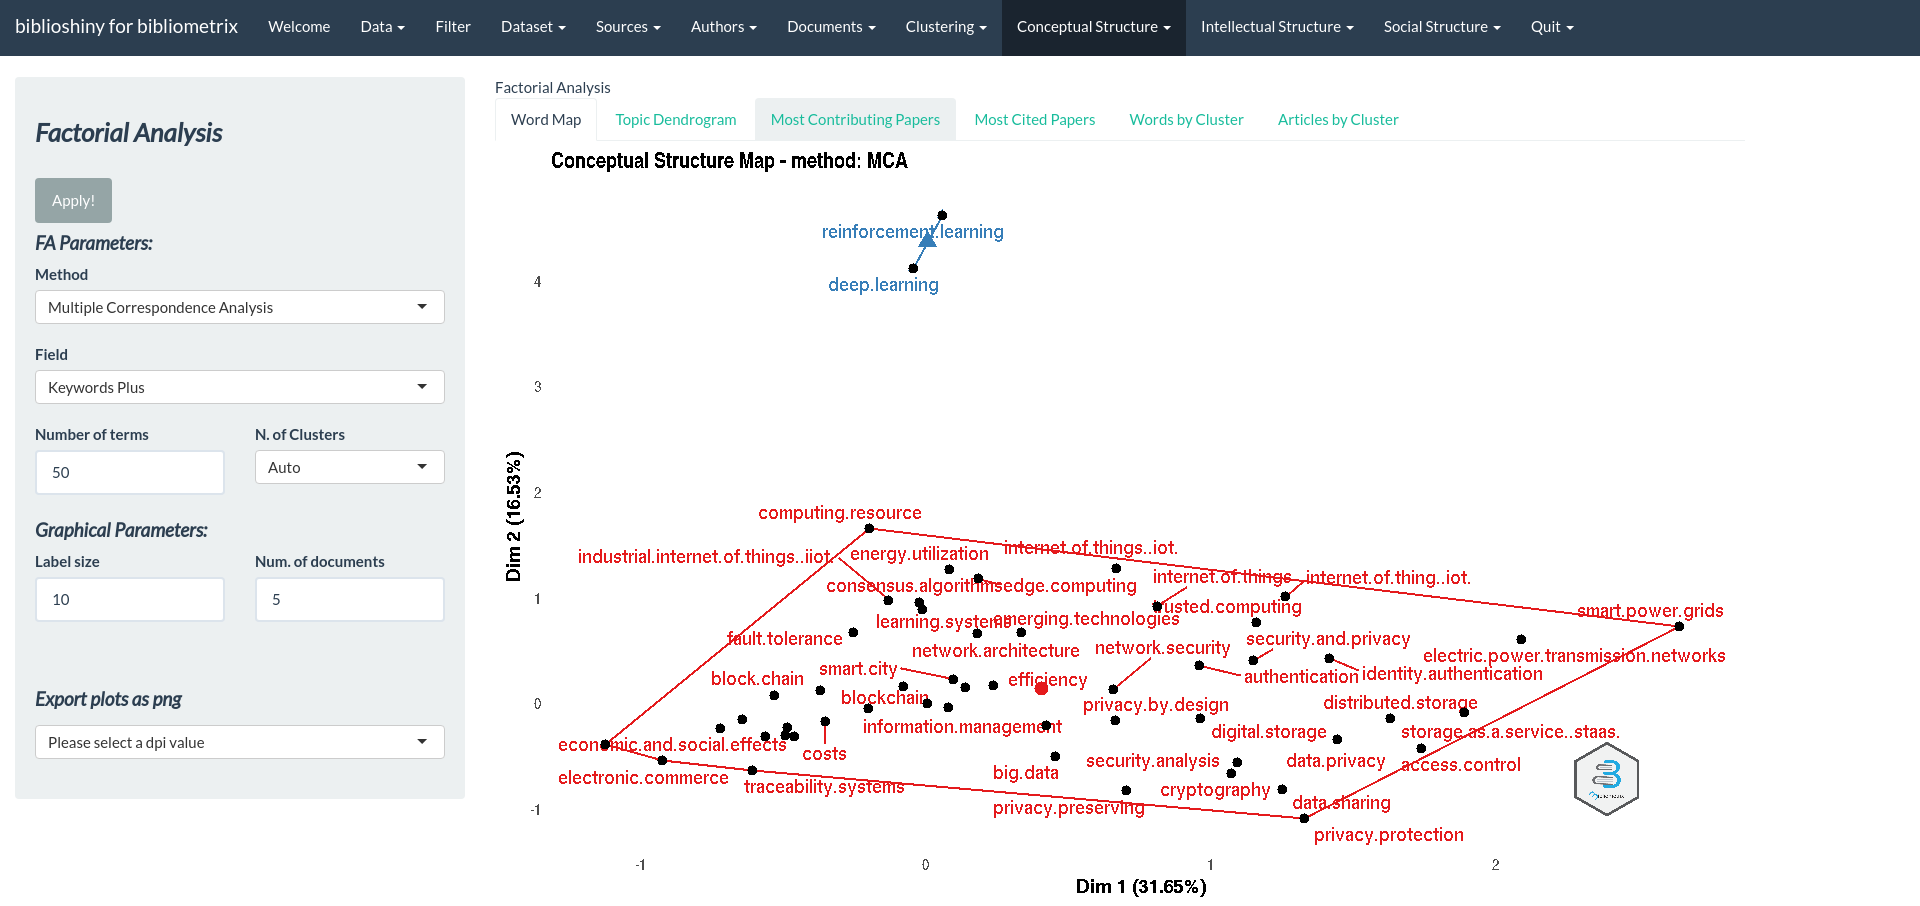
\includegraphics[width=.95\textwidth]{Result1.png}
\end{figure}  
\end{frame}

\begin{frame}{Ejemplo blockchain}
Algunos resultados
\begin{figure}
\centering
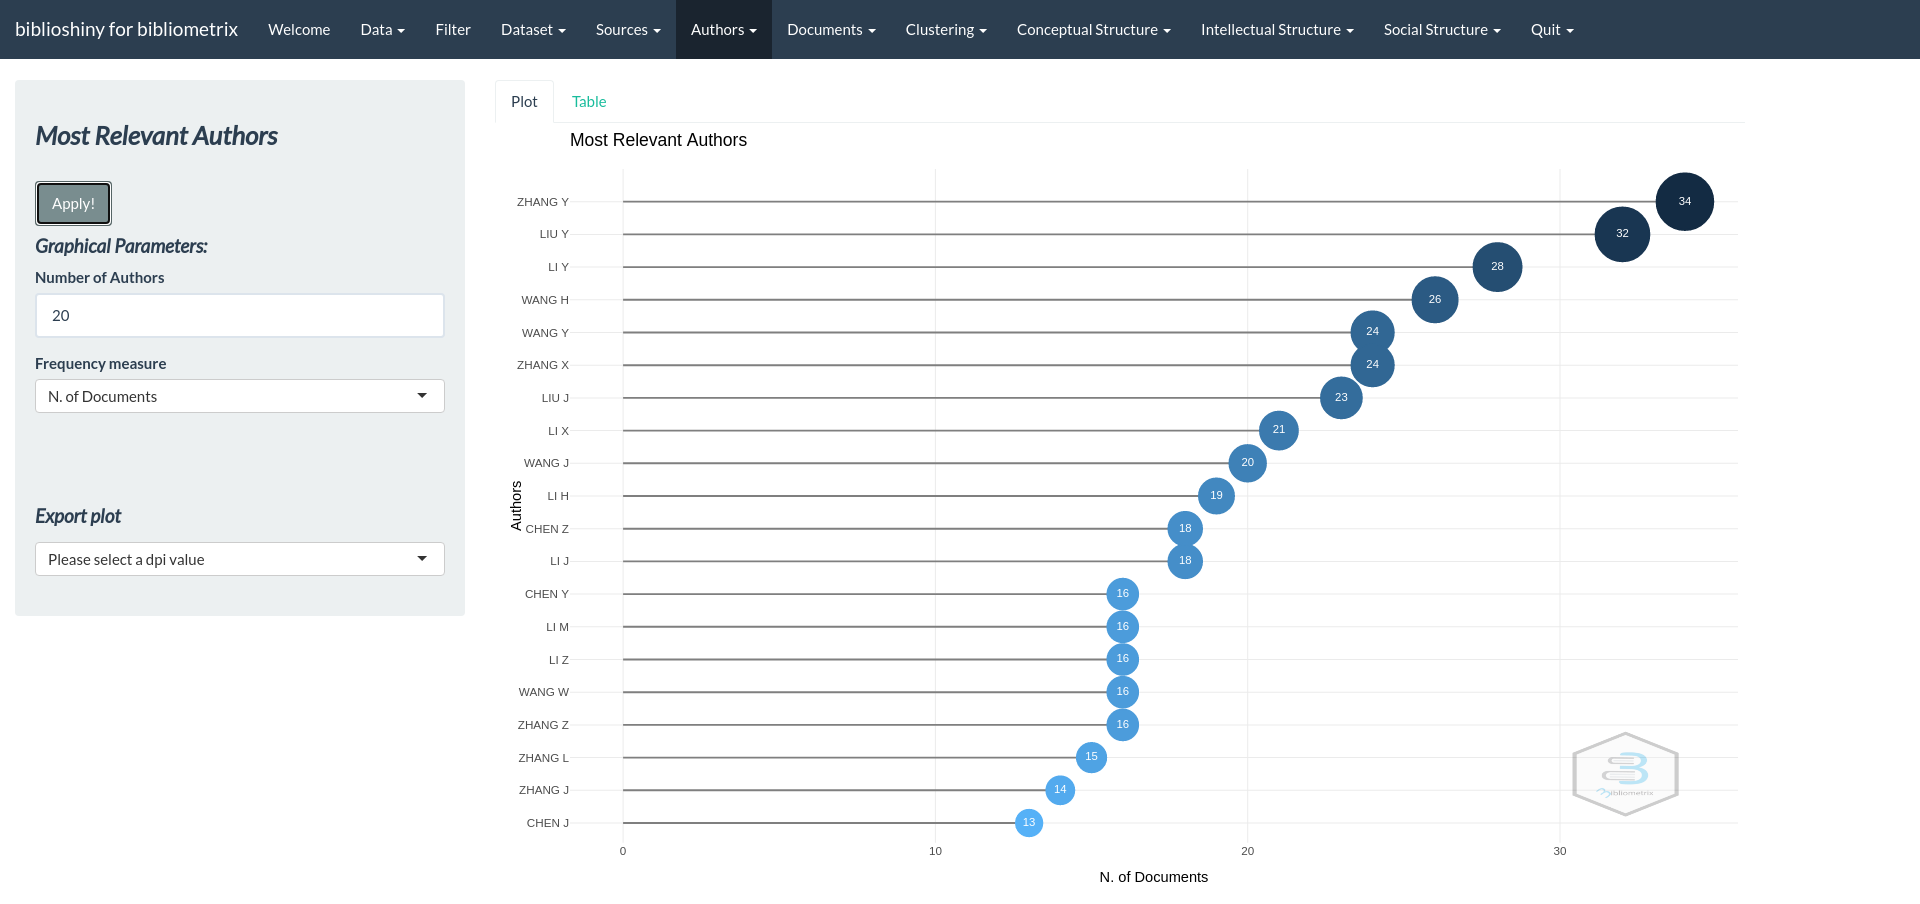
\includegraphics[width=.95\textwidth]{Result2.png}
\end{figure}  
\end{frame}

\begin{frame}{Ejemplo blockchain}
Algunos resultados
\begin{figure}
\centering
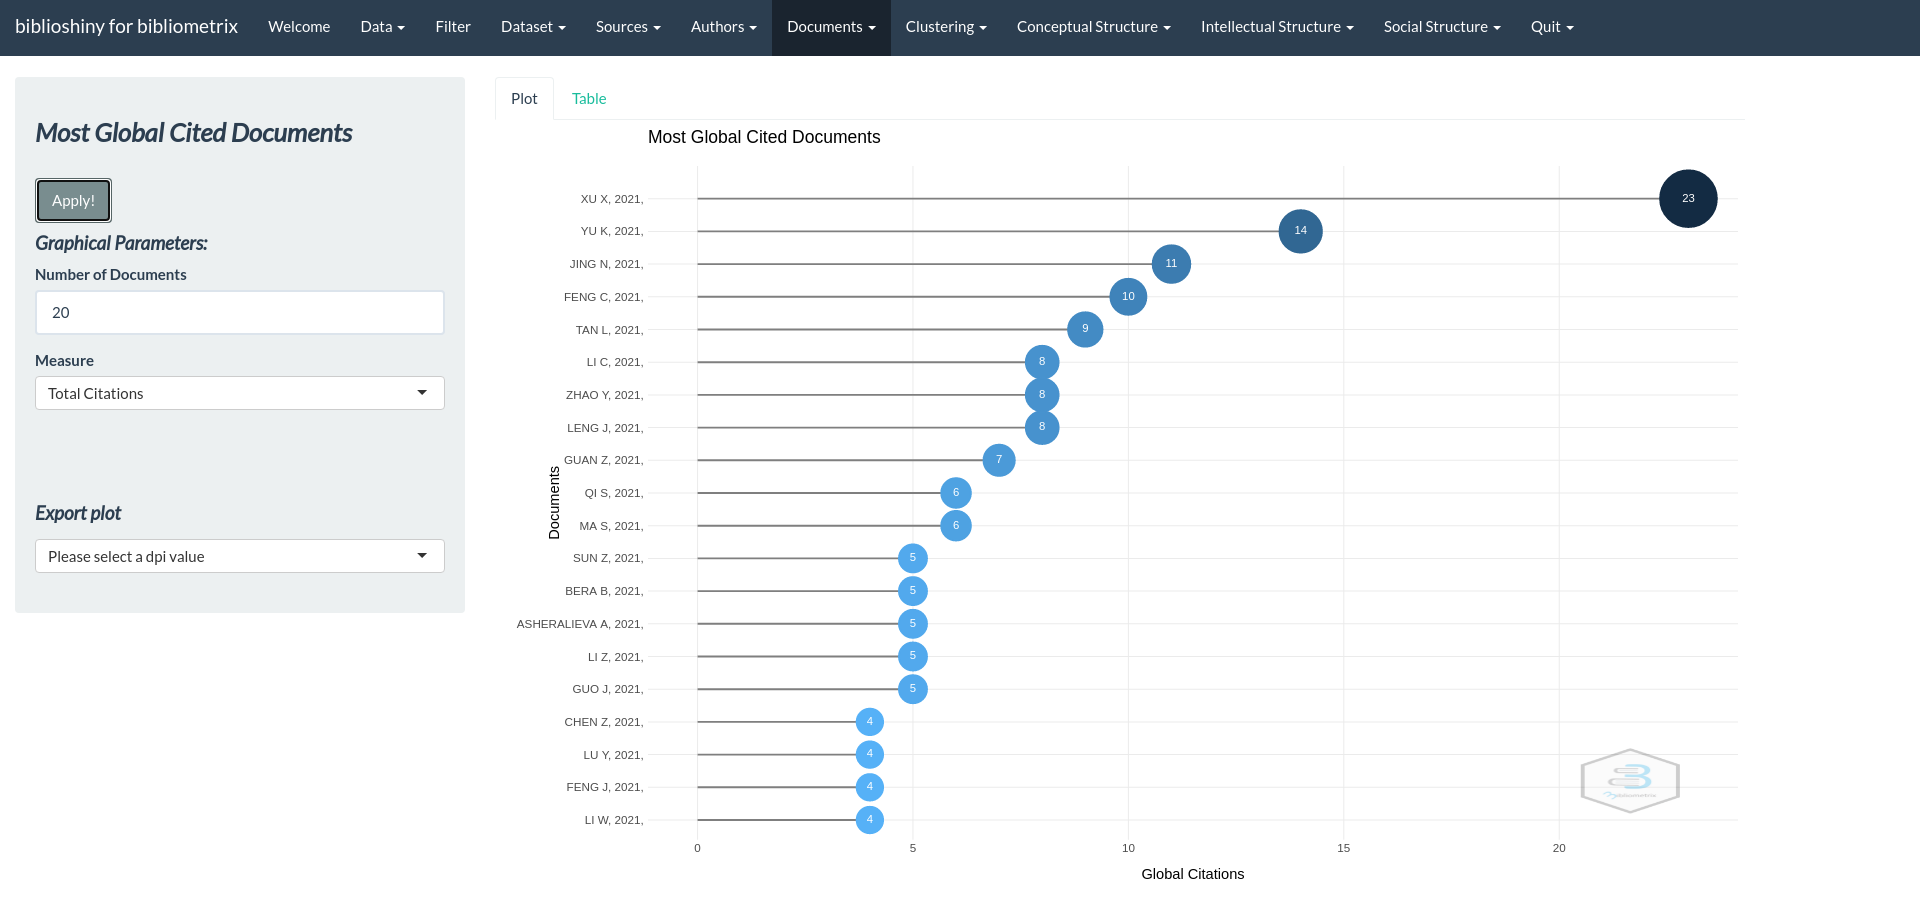
\includegraphics[width=.95\textwidth]{Result3.png}
\end{figure}  
\end{frame}

\begin{frame}{Ejemplo blockchain}
Algunos resultados
\begin{figure}
\centering
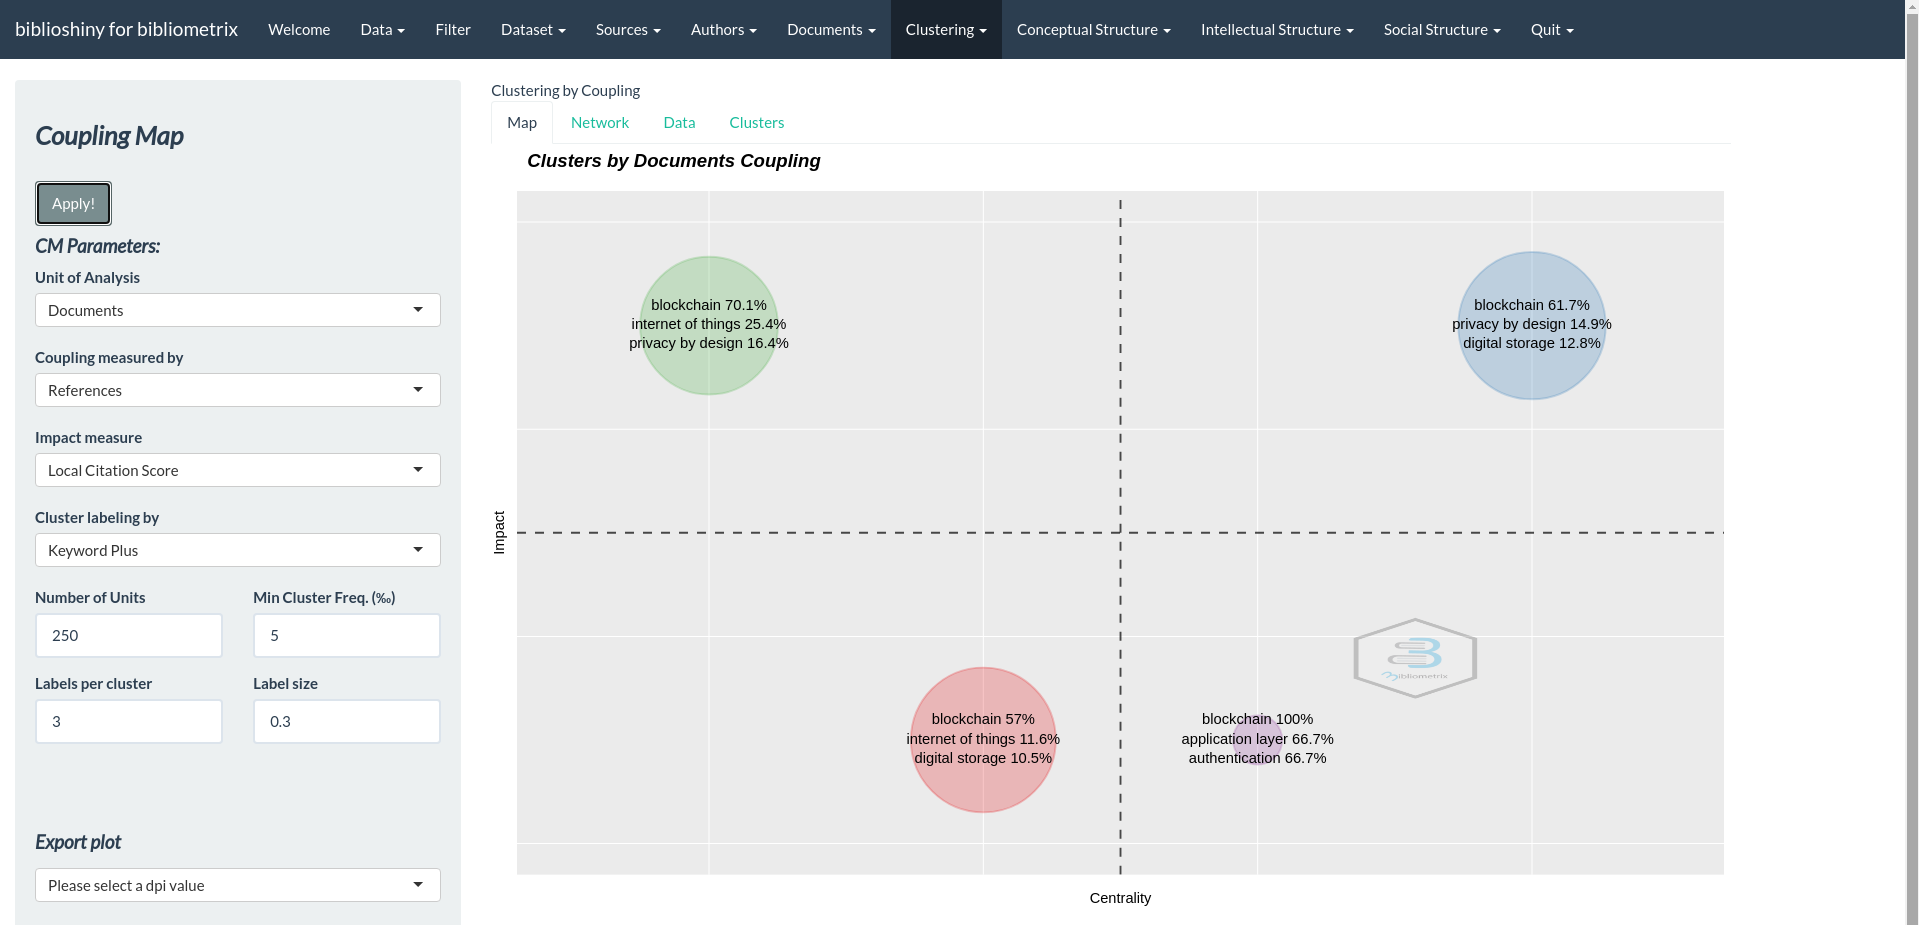
\includegraphics[width=.95\textwidth]{Result4.png}
\end{figure}  
\end{frame}

\begin{frame}{Ejemplo blockchain}
Algunos resultados
\begin{figure}
\centering
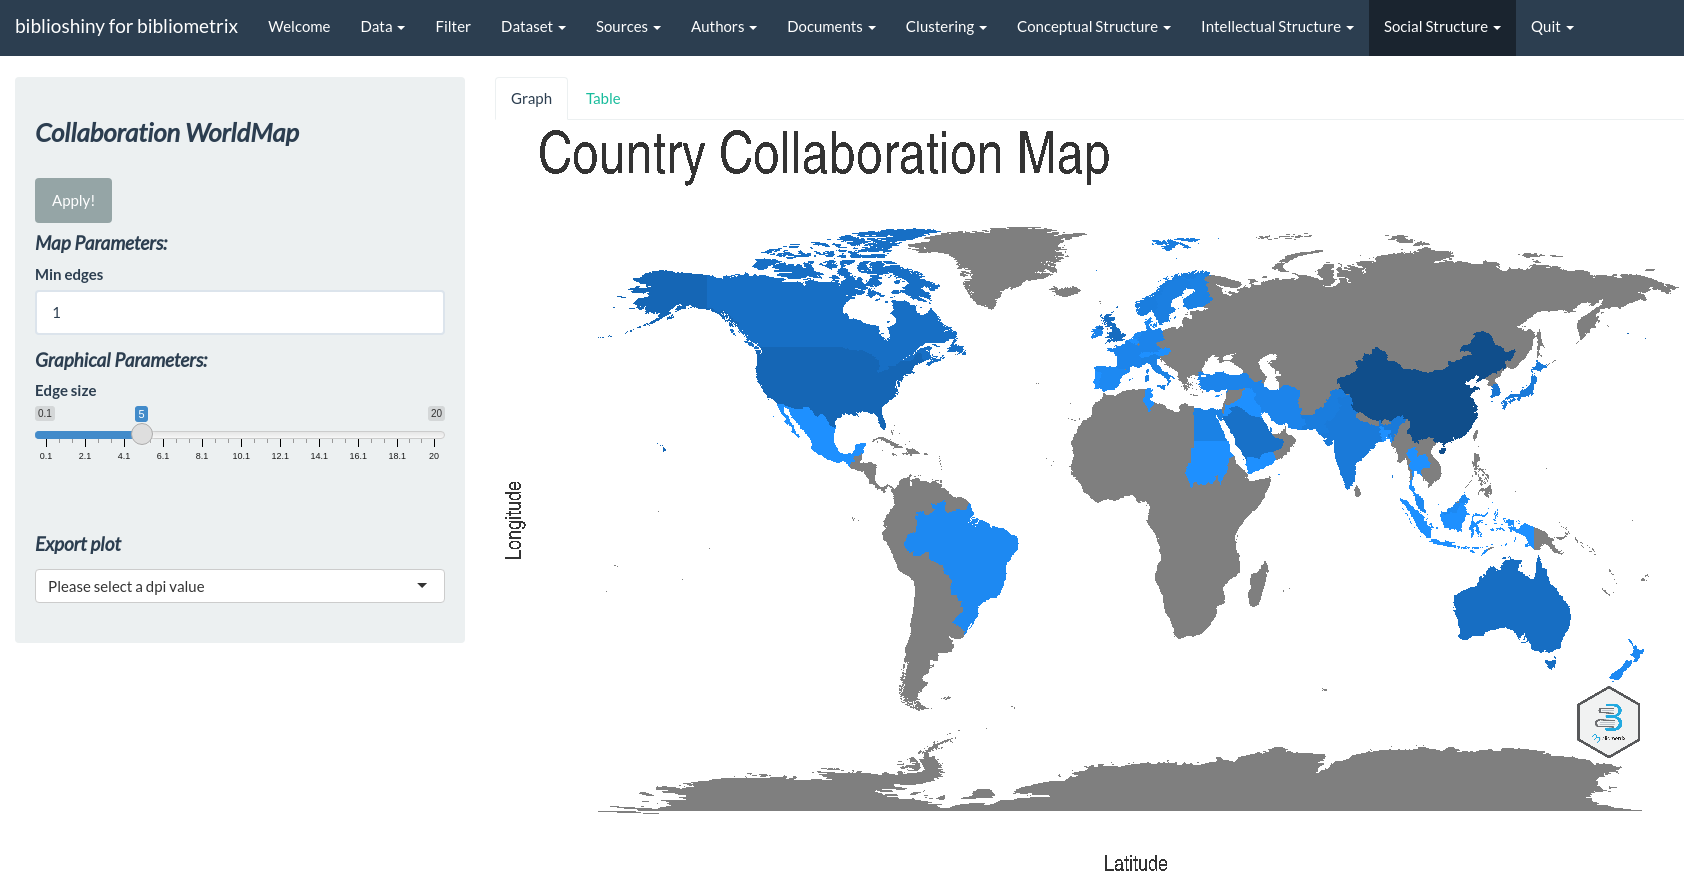
\includegraphics[width=.95\textwidth]{Result5.png}
\end{figure}  
\end{frame}


\begin{frame}[allowframebreaks]{Referencias}
\tiny{ 
\bibliographystyle{apacite}
\bibliography{refs}
}
\end{frame}


\end{document}